\documentclass[a4paper, 11pt]{article}

\usepackage[margin=1in]{geometry}
\usepackage{natbib}
\bibpunct[:]{(}{)}{,}{a}{}{;}

%--------------------
%\usepackage{gb4e}
%\noautomath

\usepackage{amsmath}
\usepackage{amsfonts}
\usepackage{amsthm}
\usepackage{amssymb}
\usepackage{mathrsfs}
\usepackage{nicefrac}
%\usepackage{stmaryrd}
%\usepackage{multicol}
\usepackage{graphicx}
\usepackage{color}
\usepackage{booktabs}
\usepackage{pgfplots}
\usepackage{subcaption}
\pgfplotsset{compat=1.3}
\usetikzlibrary{pgfplots.groupplots,decorations.markings}

\newtheoremstyle{Satz}
   {}                      %Space above
   {1em}                   %Space below
   {\normalfont}           %Body font
   {}                      %Indent amount (empty = no indent,
                           %\parindent = para indent)
   {\normalfont}           %Thm head font
   {.}                     %Punctuation after thm head
   {.8em}                  %Space after thm head: " " = normal interword
                           %space; \newline = linebreak
   {\bfseries\thmname{#1}\thmnote{ (#3)}}
                           %Thm head spec (can be left empty, meaning
                           %`normal')

\theoremstyle{Satz}
\newtheorem{example}{Example}

%\newcommand{\mvalueof}[1]{\llbracket#1\rrbracket}
\newcommand{\citeposs}[2][]{\citeauthor{#2}'s (\citeyear[#1]{#2})}
\newcommand{\tuple}[1]{\ensuremath{\left\langle #1 \right\rangle}} 

\newcommand{\hl}[1]{\textcolor[rgb]{.8,.33,.0}{#1}}% prints in orange
%\newcommand{\argmax}[1]{\underset{#1}{\operatorname{arg}\,\operatorname{max}}\;}
%\newcommand{\argmin}[1]{\underset{#1}{\operatorname{arg}\,\operatorname{min}}\;}
%\newcommand{\sbna}{\exists\lnot\forall}

\definecolor{Red}{RGB}{178,34,34}
\definecolor{Steelblue}{RGB}{70,130,180}
\newcommand{\mf}[1]{\textcolor{Red}{[MF: #1]}} 
\newcommand{\tb}[1]{\textcolor[rgb]{.8,.33,.0}{[TB: #1]}}% prints in orange
\newcommand{\rvv}[1]{\textcolor{Steelblue}{#1}}% prints in steel blue
\definecolor{indianred}{RGB}{205,92,92}
\definecolor{mygray}{cmyk}{0.35,0.35,0.35,0.35}
\definecolor{goldish}{RGB}{118, 104, 154}

\usepackage{blkarray}
\usepackage{xspace}

\usepackage{tgtermes}
\renewcommand{\baselinestretch}{1.2}

%%% MF's commands
\newcommand{\set}[1]{\left\{#1\right\}}
\newcommand{\card}[1]{\left \lvert \, #1 \, \right\rvert}
\newcommand{\abs}[1]{\lvert #1 \rvert}
\newcommand{\States}{\ensuremath{S}\xspace}		% Set of States
\newcommand{\state}{\ensuremath{s}\xspace}		% single states
\newcommand{\mystate}[1]{\ensuremath{\state_{\text{#1}}}\xspace} %meaningful states
\newcommand{\mylang}[1]{\ensuremath{L_{\text{#1}}}\xspace} %meaningful states
\newcommand{\Messgs}{\ensuremath{M}\xspace}		% Set of Messages
\newcommand{\messg}{\ensuremath{m}\xspace}		% single messages
\newcommand{\mymessg}[1]{\ensuremath{\messg_{\text{#1}}}\xspace} %meaningful messages
\newcommand{\ssome}{\mystate{\ensuremath{\exists\neg\forall}}}
\newcommand{\sall}{\mystate{\ensuremath{\forall}}}
\newcommand{\snone}{\mystate{\ensuremath{\emptyset}}}
\newcommand{\msome}{\mymessg{some}}
\newcommand{\mall}{\mymessg{all}}
\newcommand{\mnone}{\mymessg{none}}
\newcommand{\Lall}{\mylang{all}}
\newcommand{\Lbound}{\mylang{bound}}
\newcommand{\Llack}{\mylang{lack}}
\newcommand{\asome}{\myact{\ensuremath{\exists\neg\forall}}}
\newcommand{\aall}{\myact{\ensuremath{\forall}}}

\definecolor{mygray}{cmyk}{0.35,0.35,0.35,0.35}
\newcommand{\mygray}[1]{{\textcolor{mygray}{#1}}}
%%% 


%--------------------
%
\usepackage{setspace}
\doublespacing
%
%-------------------


\title{Co-evolution of lexical meaning \& pragmatic use}

% \author{%\bf NAME1 and NAME2\\
%     ( -- draft \today --- )
% }


\date{}

\begin{document}

  %% for arrow head placement
  \tikzset{->-/.style={decoration={
  markings,
  mark=at position #1 with {\arrow{>}}},postaction={decorate}}}
  %%% 

\maketitle

\begin{abstract}
 According to standard linguistic theory, the meaning of an utterance is the product of
  conventional semantic meaning and general pragmatic rules on language use. To investigate how
  cultural evolution of language plays out under this picture of the semantics-pragmatics
  interface, we present a game-theoretic model of the competition between types of language
  users, each endowed with a selection of lexical representations and a particular pragmatic
  disposition to act on them. Our model traces two evolutionary forces and their interaction:
  (i) pressure towards communicative efficiency and (ii) transmission perturbations during the acquisition of
  linguistic knowledge. We illustrate the model based on a case study on scalar
  implicatures, which suggests the relationship between underspecified semantics and pragmatic inference to be one of co-evolution. The maintenance of underspecified semantics depends on pragmatic reasoning for their enrichment. In the opposite direction, complex semantics that can do away with mutual reasoning may not foster pragmatic reasoning, and may even be encumbered by it.
\end{abstract}

\section{Introduction}\label{sec:introduction}

What is conveyed usually goes beyond what is said. A request for a blanket can be politely
veiled by uttering ``I'm cold;'' a temporal succession of events can be communicated by the order
in which conjuncts appear as in ``I traveled to Paris and got married;'' an invitation can be
declined by saying ``I have to work.'' An influential explanation of the relation between the
literal meaning of expressions and what they may convey in context is due to
\citet{grice:1975}, who characterizes pragmatic use and interpretation as a process of mutual
reasoning about rational language use. For instance, under the assumption that the speaker is
cooperative and relevant, ``I have to work'' may be interpreted as providing a reason why the
speaker will not be able to accept an invitation, going beyond its literal meaning. Some of
these enrichments are rather \emph{ad hoc}. Others show striking regularities, such as the use
of ability questions for polite requests (``Could you please \dots?''), or certain enrichments
of lexical meanings such as \emph{and} to convey \emph{and then}.

A particularly productive and well studied class of systematic pragmatic enrichments are scalar
implicatures
\citep{horn:1984,Hirschberg1985:A-Theory-of-Sca,LevinsonPragmatics1983,Geurts2010:Quantity-Implic}. Usually,
the utterance of a sentence like ``I own some of Johnny Cash's albums'' will be taken to mean
that the speaker does not own all of them. This is because, if the speaker instead owned them all, she
could have used the word \emph{all} instead of \emph{some} in her utterance, thereby making a
more informative statement. Scalar implicatures, especially the inference from \emph{some} to
\emph{some but not all}, have been studied extensively, both theoretically
\citep[e.g.,][]{Sauerland2004:Scalar-Implicat,ChierchiaFox2008:The-Grammatical,Rooyvan-RooijJagerde-Jager2012:Explaining-Quan}
as well as experimentally
\citep[e.g.,][]{BottNoveck2004:Some-Utterances,huang+snedeker:2009,GrodnerKlein2010:Some-and-Possib,GoodmanStuhlmuller2013:Knowledge-and-I,DegenTanenhaus2012:Processing-Scal}. This makes them particularly suitable candidates for the study of the evolution of regular pragmatic inferences.  While there is much dispute in this domain about many details, a position endorsed by a clear majority is that a scalar item like \emph{some} is underspecified to mean \emph{some and maybe all} and that the enrichment to \emph{some but not all} is part of some regular process with
roots in pragmatics.

If this majority view is correct, the question arises how such a division of labor between
semantics and pragmatics could have evolved; why it would be so pervasive across natural
languages; and why it is that some expressions systematically draw from it while others semantically conventionalize. 

Models of language evolution abound. There are simulation-based models studying
populations of communicating agents
\citep{Hurford1989:Biological-Evol,Steels1995:A-Self-Organizi,LenaertsJansen2005:The-Evolutionar,SteelsBelpaeme2005:Coordinating-Pe,BaronchelliPuglisi2008:Cultural-route-,steels:2011,SpikeStadler2016:Minimal-Require}
and there are mathematical models of language evolution, many coming from game theory
\citep{Warneryd1993:Cheap-Talk-Coor,BlumeKim1993:Evolutionary-St,nowak+krakauer:1999,nowak:2006,Huttegger2007:Evolution-and-t,Skyrms2010:Signals}. Much
of this work has focused on explaining basic properties such as compositionality and
combinatoriality
\citep[e.g.,][]{Batali1998:Computational-S,nowak+krakauer:1999,nowak+etal:2000,KirbyHurford2002:The-Emergence-o,kirby:2002,SmithKirby2003:Iterated-Learni,Gong2007:Language-Evolut,kirby+etal:2015,verhoef+etal:2014,Franke2015:Proto-Syntax},
but little attention has been paid to the interaction between conventional meaning and
pragmatic use. What is more, many mathematical models explain evolved meaning as a regularity
in the overt behavior of agents, abstracting from complex interactions between semantic
representations and pragmatic use. In contrast, we will here look at language users with a
richer linguistic make-up. More precisely, we spell out a model of the evolution of conventional meaning and pragmatic reasoning.
The objects of replication and selection are pairs consisting of a set of lexical
meanings and a manner of pragmatic behavior, which together define agents' linguistic choices. Pragmatic behaviors are represented using probabilistic models of pragmatic language use \citep{frank+goodman:2012,FrankeJager2015:Probabilistic-p,GoodmanFrank2016:Pragmatic-Langu}. Replication
and selection are described by the \emph{replicator mutator dynamic}, a general and established
model of evolutionary change in large and homogeneous populations
\citep{Hofbauer1985:The-Selection-M,nowak+etal:2000,NowakKomarova2001:Evolution-of-Un,hofbauer+sigmund:2003,nowak:2006}. This
approach allows us to study the interaction between (i) pressure towards communicative
efficiency and (ii) infidelity in the transmission of linguistic knowledge, caused by factors
such as inductive learning biases and sparse learning data \citep{KirbyHurford2002:The-Emergence-o,SmithKirby2003:Iterated-Learni,KirbyGriffith2014:Iterated-Learni}. Considering the effects that the transmission of
linguistic knowledge through (iterated) learning have is important because neither semantic meaning nor pragmatic usage
patterns are directly observable. Instead, language learners have to infer these unobservables from the observable behavior in which they result. We formalize this process as a form of
Bayesian inference. Our approach thereby contains a well-understood model of
iterated Bayesian learning \citep{griffiths+kalish:2005,griffiths+kalish:2007}, but combines it with functional
selection, here formalized as the most versatile dynamic from evolutionary game theory, the
replicator dynamic \citep{TaylorJonker1978:Evolutionary-St}. Section~\ref{sec:model} introduces
this model.

Section~\ref{sec:si-case-study} applies this model to a case study on scalar implicatures. We
discuss a setting in which the majority view of underspecified lexical meanings and systematic pragmatic
enrichments emerges if selection and transmission infidelity are combined. In particular, we
show that inductive learning biases of Bayesian learners that favor simpler lexical meanings
may play a role in preventing the lexicalization of scalar inferences and thereby lead to the emergence of Gricean-like
pragmatic reasoning types. The results of this study are critically assessed in the light of
the assumptions that feed our model in Section~\ref{sec:discussion}.

% We see the main contribution of this work as conceptual and technical, not as a definite answer
% to the question why scalar implicatures emerge. It rather demonstrates how current
% probabilistic cognitive modeling of language use and evolutionary modeling can be fruitfully
% combined to study the co-evolution of semantics and pragmatics side-by-side. Reversely, the
% approach taken here may be seen as a first step towards giving an evolutionary rationale for
% empirically successful probabilistic models of language use that embrace the majority view of
% the division of labor between semantics and pragmatics. Section~\ref{sec:discussion} elaborates
% on these points.

\section{A model of evolving lexical representations and pragmatic behavior}
\label{sec:model}

\subsection{Communicative success and learnability}

The emergence and change of linguistic structure is influenced by many intertwined
factors. These range from biological and socio-ecological to cultural ones \citep{benz+etal:2005b,steels:2011,tamariz+kirby:2016}. Social and ecological pressures determine communicative needs, while
biology determines the architecture that enables and constrains the means by which they can be
fulfilled. In the following, our focus lies on cultural aspects, wherein processes of
linguistic change are viewed as shaped by language use and its transmission, i.e., as a result
of a process of cultural evolution
\citep{Pagel2009:Human-Language-,ThompsonKirby2016:Culture-Shapes-}.

The idea that language is an adaptation to serve a communicative function is fundamental to
many synchronic and diachronic analyses, at least since \citeposs{zipf:1949} explanation of word
frequency rankings as a result of competing hearer and speaker preferences \citep[e.g.,
in][]{martinet:1962, horn:1984,jaeger+vRooij:2007,jaeger:2007,
  piantadosi:2014,kirby+etal:2015}. If processes of selection, such as conditional imitation or
reinforcement, favor more communicatively efficient types of behavior, languages are driven
towards semantic expressivity \citep[e.g.,][]{nowak+krakauer:1999,Skyrms2010:Signals}. But
pressure towards communicative efficiency is not the only force that shapes
language. Learnability is another, as natural languages need to be learnable to survive their
faithful transmission across generations. Furthermore, the effects of even small learning biases implicit in acquisition can build up and have quite striking impact on an evolving language in a process of iterated
learning
\citep{KirbyHurford2002:The-Emergence-o,SmithKirby2003:Iterated-Learni,kirby+etal:2014}.

While natural languages are pressured for both communicative efficiency and learnability, these forces may
pull in opposite directions \citep[\S7]{christiansen+chater:2008}. Their opposition becomes particularly clear when considering the
extreme (\citealt{kemp+regier:2012,kirby+etal:2015}). A language consisting of a single
form-meaning association is easy to learn but likely bad for communication with peers. Conversely, a language
that lexicalizes distinct forms for a large number of different meanings may be better for communication 
but challenging to acquire.

\subsection{The replicator mutator dynamic}
An elegant formal approach to capture the interaction between communicative efficiency and
learnability is the \emph{replicator mutator dynamic}
\citep{Hofbauer1985:The-Selection-M,nowak+etal:2000,NowakKomarova2001:Evolution-of-Un,hofbauer+sigmund:2003,nowak:2006}. The
RMD is a population dynamic, which is to say that it describes change in the composition of a
community made up of different types of agents. The population vector $\vec{x}$ codifies
relative frequencies of types in a population, where $x_i$ is the relative frequency of type
$i$ and $\sum\nolimits_i x_i = 1$. The dynamic assumes a virtually infinite population, so that
it is able to abstract away from what individual agents do and how they change their behavior
over time. The result is an abstract description of the most probable trajectory of change in
$\vec{x}$. In its simplest, discrete-time formulation, the RMD defines the frequency $x'_i$ of
each type $i$ in a population at the next time step as a function of: (i) the frequency $x_i$
of each type $i$ before the update step, (ii) the fitness $f_i$ of each type $i$ before the
update, and (iii) the probability $Q_{ji}$ that an agent who observes the behavior of an agent
with type $j$ ends up acquiring type $i$:
\begin{align}
  \label{eq:RMD_discrete}
  x'_i = \sum_j Q_{ji} \frac{x_jf_j}{\sum_h x_h f_h}\,.
\end{align}
The RMD consists of two components: fitness-based selection and transmission biases encoded in the so-called mutation matrix $Q$. This
becomes most transparent when we consider an equivalent formulation in terms of a step-wise
application of the discrete-time replicator dynamic \citep{TaylorJonker1978:Evolutionary-St} on the initial population vector $\vec{x}$ and its subsequent multiplication with the mutation matrix $Q$:
\begin{align}
  \label{eq:RMD_discrete_recast}
  x'_i & = (\text{M}(\text{RD}(\vec{x})))_i\,,
\end{align}
where
\begin{align*}
      \left ( \text{RD}(\vec{x}) \right )_i 
         = \frac{x_i f_i}{\sum_k x_k f_k}
 \ \ \ \ \text{and} \ \ \ \ 
  (\text{M}(\vec{x}))_i = (\vec{x} \cdot Q)_i = \left ( \sum_j
          x_j Q_{ji} \right)_i\,.
\end{align*}
%

If the transmission matrix $Q$ is trivial in the sense that $Q_{ji}=1$ whenever $j=i$, the
dynamic reduces to the replicator dynamic. This situation is one where types are always replicated faithfully. The replicator dynamic is a model of fitness-based selection in which the relative frequency of type $i$ will increase with a gradient proportional to its average fitness in the population. In other words, selection comes into play whenever two or more types replicate at different rates due to differences in their fitness. This dynamic is popular and versatile because it can be derived from many abstract processes of biological and cultural
transmission and selection \citep[for overview and several derivations
see][]{Sandholm2010:Population-Game}, including conditional imitation
\citep[e.g.,][]{Helbing1996:A-Stochastic-Be,Schlag1998:Why-Imitate-and} or reinforcement
learning \citep[e.g.,][]{BorgersSarin997:Learning-Throug,Beggs2005:On-the-Converge}. If fitness
$f_i$ is the same for all types $i$, the replicator step is the identity map
$ \left ( \text{RD}(\vec{x}) \right )_i = x_i$. In words, no difference in fitness translates into a lack of functional pressure: the population's type composition stays the same after the replicator step. In such cases the dynamic reduces to a process of iteration of the transmission bias encoded in $Q$: the rate by which one type changes into another after a generational turnover. As detailed below, in this way, the process in (\ref{eq:RMD_discrete}), and its equivalent in (\ref{eq:RMD_discrete_recast}), can contain a model of iterated learning \citep{griffiths+kalish:2005,griffiths+kalish:2007}. 

\begin{figure}[t]
  \centering
  %% notice that the figure is hacked, because somehow the curve does not come out right under
  %% PGFplots; I don't know why!?!?
  

    \begin{subfigure}[b]{0.45\textwidth}
      \centering
      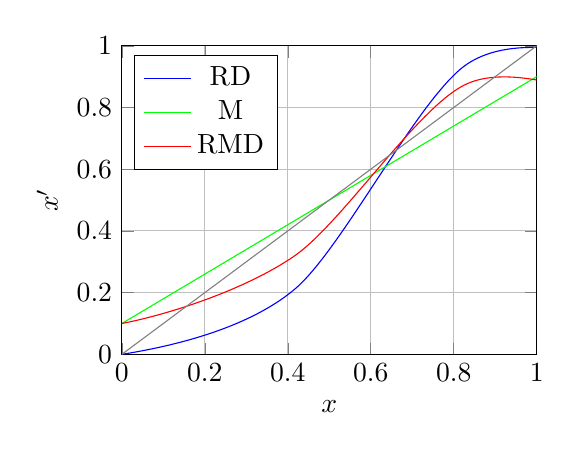
\begin{tikzpicture}
      \begin{axis}[xlabel=$x$, ylabel = $x'$,
                   grid=major, width=6.85cm, height = 5.5cm,
                   legend style = {legend pos = north west},
                   ymin=0,ymax=1, xmin=0,xmax=1]

      \addplot[smooth, color=blue] {x^2 / (3*x^2 - 4*x + 2) + 0.019 * x};
      \addplot[smooth, color=green] {.8*x + .1};

      \addplot[smooth, color=red] {(.9*x^2 - .2*x +.2)/(3*x^2 - 4*x + 2)};

      \addplot[smooth, color=gray] {x};

      \legend{RD, M, RMD}

      \end{axis}
    \end{tikzpicture}


        \caption{Update functions: the population state $x$ is mapped onto $x'$ in one update step.}
        \label{fig:Updates_RMS}
    \end{subfigure}
    \hfill
    \begin{subfigure}[b]{0.5\textwidth}    
      \centering
    \begin{tikzpicture}[x=120]
      \node[draw=black, circle, fill = black, minimum size = 0.25cm]
      (0) at (0,0) {};

      \node[draw=black, circle, fill = black, minimum size = 0.25cm]
      (1) at (1,0) {};

      \draw[-, thick] (0) -- (1);

      \node[draw=black, circle, fill = white, minimum size = 0.25cm, thick]
      (mid) at (2/3,0) {};

      \node[]  (0.label) at (0,-0.5) {0};

      \node[]  (1.label) at (1,-0.5) {1};

      \node[]  (label) at (0.5,-0.5) {$x$};

      \node[]  (label) at (0.5,0.55) {RD};

      \draw[->-=0.8,very thick] (mid) -- (0);

      \draw[->-=0.8,very thick] (mid) -- (1);

    \end{tikzpicture}
    
    \vspace*{0.35cm}

    \begin{tikzpicture}[x=120]

      \node (0) at (-0.05,0) {};

      \node (1) at (1.05,0) {};

      \draw[-, thick] (0) -- (1);

      \node[draw=black, circle, fill = black, minimum size = 0.25cm, thick]
      (mid) at (0.5,0) {};

      \node[]  (0.label) at (0,-0.3) {0};

      \node[]  (1.label) at (1,-0.3) {1};

      \node[]  (label) at (0.5,-0.5) {$x$};

      \node[]  (label) at (0.5,0.55) {M};

      \draw[->-=0.5,very thick] (0) -- (mid);

      \draw[->-=0.5,very thick] (1) -- (mid);

    \end{tikzpicture}

    \vspace*{0.35cm}

    \begin{tikzpicture}[x=120]

      \node (0) at (-0.05,0) {};

      \node (1) at (1.05,0) {};

      \node[draw=black, circle, fill = black, minimum size = 0.25cm]
      (S0) at (0.121,0) {};

      \node[draw=black, circle, fill = black, minimum size = 0.25cm]
      (S1) at (0.903,0) {};

      \draw[-, thick] (0) -- (1);

      \node[draw=black, circle, fill = white, minimum size = 0.25cm, thick]
      (mid) at (0.609,0) {};

      \node[]  (0.label) at (0,-0.3) {0};

      \node[]  (1.label) at (1,-0.3) {1};

      \node[]  (label) at (0.5,-0.5) {$x$};

      \node[]  (label) at (0.5,0.55) {RMD};

      \draw[->-=0.5,very thick] (mid) -- (S0);

      \draw[->-=0.5,very thick] (mid) -- (S1);

      \draw[->-=0.5,very thick] (0) -- (S0);

      \draw[->-=0.5,very thick] (1) -- (S1);

    \end{tikzpicture}
        


    \caption{Phase portraits for RD, M and RMD: unstable rest points are hollow, attractors are
      solid.}
        \label{fig:Phase_RD}
    \end{subfigure}

  \caption{Example.}
  \label{fig:Example_RMD}
\end{figure}

\begin{example}
  Consider a simple and abstract coordination game. Agents are of two types: positive or negative. If
  agents of different type interact with each other, they obtain a payoff of $0$. If negative meets
  negative, each receives a payoff of $1$. If positive meets positive, they get a payoff of $2$.  A population state is completely characterized by the proportion $x$ of negatives. The fitness
  of negatives in population state $x$ is $f_n(x) = x$, that of positives is $f_p(x) = 2-2x$.
  The average fitness is $\Phi(x) = x f_n(x) + (1-x) f_p(x) = 3x^2 - 4x + 2$. Without mutation,
  the replicator dynamic will update $x$ to $\text{RD}(x) = \nicefrac{f(x)x}{\Phi(x)} = \nicefrac{x^2}{\Phi(x)}$. The update
  function $\text{RD}(x)$ of the replicator step is plotted in Fig.~\ref{fig:Updates_RMS} as the
  blue line. Rest points, for which $\text{RD}(x)=x$, are at $x=0$, $x=1$ and $x= \nicefrac{2}{3}$.
  The former are attractors; nearby points converge to them. Points near $x=\nicefrac{2}{3}$
  also move towards 0 or 1. This is schematically pictured in the topmost phase portrait in
  Fig.~\ref{fig:Phase_RD}. Adding mutation changes the dynamic and its rest points. Let us assume that $Q_{ji} = .9$
  when $j=i$. This is the proportion of types that are replicated faithfully. Conversely, a proportion of $.1$ will change their type from positive to negative, and vice-versa. The update effect of mutation on its own are described by $\text{M}(x) = .9 x + .1 (1-x) = .8x + .1$, plotted as the linear green line in Fig.~\ref{fig:Updates_RMS}. As shown in Fig.~\ref{fig:Phase_RD}, in this example mutation alone has only one stable rest point. It is located at $x = .5$. If we first take the replicator step and
  then the mutation step in sequence, we obtain the replicator mutator dynamic
  $\text{RMD}(x) = \text{M}(\text{RD}(x)) = \nicefrac{.9x^2 - .2x +.2}{3x^2 - 4x + 2}$, which is plotted in red in
  Fig.~\ref{fig:Updates_RMS}. The rest points are at $x=.121$, $x=.903$ and $x=.609$. The
  former two are attractors (see Fig.~\ref{fig:Phase_RD}).
\end{example}




\subsection{Fitness \& learnability of lexical meanings \& pragmatic strategies}
\label{sec:fitn--learn}


Moving beyond an abstract example, our goal is to apply the RMD to investigate the evolution
of lexical representations and pragmatic behavior. To do so, we need to fix three things: (i) what the
relevant types are that populate $x$, (ii) how fitness derives from communicative success and (iii) how the
mutation matrix $Q$ is computed. These issues are addressed, one by one, in the following.

\subsubsection{Types: Lexica and pragmatic strategies}
\label{sec:languages+use}
Types are what evolution operates on. They define an agent's fitness, usually through a payoff
accrued in single interactions with other agents. Often types can be identified as the possible
acts in a game, e.g., either cooperating or defecting in a prisoner's dilemma. In other cases,
they may be thought of as general properties of an agent that influence her fitness, such as
being positive or negative in our previous example (whatever that means). For our present
purposes, types are identified by specific assumptions about their cognitive
make-up. More concretely, since we are interested in the evolutionary competition between different lexical representations and ways of deploying them in communication, a type is here defined as a pair consisting of a lexicon and a linguistic strategy of language use.

Agents play signaling games, in which the speaker wants to communicate a world state $s$ with a
message $m$ to a hearer who receives $m$ but does not know $s$
\citep[e.g.][]{lewis:1969,Skyrms2010:Signals}. A lexicon associates each message with a
(possibly fuzzy) set of states. A linguistic behavior specifies a probabilistic speaker
rule (a probabilistic choice of message for each state) and a probabilistic hearer rule (a
probabilistic choice of state for each message) given a lexicon. There are many ways of making these general notions concrete. There are models of rational language use coming from a game-theoretic tradition \citep[e.g.,][]{benz:2006,benz+vRooij:2007,jaeger:2007b,franke+jaeger:2014} and ones from a Bayesian tradition \citep[e.g.,][]{frank+goodman:2012,goodman+stuhlmueller:2013,GoodmanFrank2016:Pragmatic-Langu}. We will not focus on the particular design choices that make up each approach (on this see \citealt{qing+franke:2015}). Instead, we will stress how the approach, common to all of these models, of pragmatic language use as {\em rational language use} can be embedded within the replicator mutator dynamic to answer evolutionary questions at the semantics-pragmatics interface. Here is what we will assume in the remainder of this paper.\footnote{Readers more familiar with the Bayesian tradition than the game-theoretic one should note that the definitions below follow the latter in assuming rational sender choice to consist in sending messages that maximize expected utility, rather than message informativity (see \citealt{qing+franke:2015} for discussion).}

Lexica codify the truth-conditions of expressions. A convenient way to represent lexica is by
$(\card{\States}, \card{\Messgs})$-Boolean matrices, where $\States$ is a set of states
(meanings) and $M$ a set of messages (forms available in the language). For example, suppose
that there are two relevant world states $\States = \set{\ssome, \sall}$. In state $\ssome$
Chris owns some but not all of Johnny Cash's albums while in $\sall$ Chris owns them
all. Suppose that there are two messages $\Messgs = \set{\msome, \mall}$ where $\msome$ is
short for a sentence like \emph{Chris owns some of Johnny Cash's albums} and $\mall$ for the
same sentence with \emph{some} replaced by \emph{all}.  Lexica for this case would assign a
Boolean truth value, either $0$ for false or $1$ for true, to each state-message pair. The
following two lexica are minimal examples for the distinction between a lexicalized upper-bound
for \emph{some}, in $\Lbound$, and the widely assumed logical semantics with only a lower-bound,
in $\Llack$.

\begin{align*}
  \Lbound & = \begin{blockarray}{lcc}
    & \mygray{\msome} & \mygray{\mall} \\
    \begin{block}{l[cc]}
      \mygray{\ssome} & 1 & 0 \\
      \mygray{\sall}  & 0 & 1 \\
    \end{block}
  \end{blockarray} &
  \Llack & = \begin{blockarray}{lcc}
    & \mygray{\msome} & \mygray{\mall} \\
    \begin{block}{l[cc]}
      \mygray{\ssome} & 1 & 0 \\
      \mygray{\sall}  & 1 & 1 \\
    \end{block}
  \end{blockarray}
\end{align*}

Linguistic strategies define dispositions to produce and interpret messages given a lexicon. We
distinguish between two kinds strategies. {\em Literal interlocutors} produce and
interpret messages literally, being guided only by their lexica. {\em Pragmatic interlocutors}
instead engage in mutual reasoning to inform their choices. Recent probabilistic models of
rational language use
\citep{frank+goodman:2012,FrankeJager2015:Probabilistic-p,GoodmanFrank2016:Pragmatic-Langu}
capture different types of pragmatic behavior in a reasoning hierarchy. The hierarchy's bottom,
level $0$, corresponds to literal language use, as in Equations~(\ref{h:level0}) and
(\ref{s:level0}). Pragmatic language users of level $n + 1$ act (approximately) rational with
respect to level-$n$ behavior of their interlocutors, as in Equations~(\ref{h:leveln}) and
(\ref{s:leveln}).
\begin{alignat}{3}
&H_{0}(s \mid m;L) &&\propto pr(s) L_{[s,m]} \label{h:level0}\\
&S_{0}(m \mid s;L) &&\propto \exp(\lambda \; L_{[s,m]}) \label{s:level0}\\
&H_{n+1}(s|m;L) &&\propto pr(s) S_{n}(m|s;L) \label{h:leveln}\\
&S_{n+1}(m|s;L) &&\propto  \exp(\lambda \; H_{n}(s|m;L)) \label{s:leveln}
\end{alignat}

According to (\ref{h:level0}), a literal hearer's interpretation of a message depends on her
lexicon and her prior over states, $pr \in \Delta(S)$, which is here assumed flat for
simplicity. Literal interpreters thereby choose an arbitrary true interpretation for each
message according to their lexicon. Pragmatic hearers, defined in (\ref{h:leveln}), instead use Bayes' rule to weigh
interpretations based on a conjecture about speaker behavior. Speaker behavior is regulated by
a soft-max parameter $\lambda \geq 0$ \citep{luce:1959,sutton+barto:1998}. As
$\lambda$ increases, choices approximate strict maximization of expected utilities. Expected
utility of a message $\messg$ in state $\state$ for a level $n+1$ speaker is here defined as
$H_{n}(s|m;L)$, the probability that the hearer will assign to or choose the correct
meaning. For literal speakers, utility only tracks truthfulness. Literal speakers choose any
true message with equal probability but may send false messages as well with a probability
dependent on $\lambda$.

In words, an agent's linguistic behavior -- what message to send when or which message to interpret how -- is defined by (i) her reasoning level and (ii) her lexicon. In what follows, this is what we identify an agent's type with, in order to analyze under which conditions combinations of (i) and (ii) emerge through cultural evolution. Intuitively, literal behavior (level-$0$ reasoning) results from unreflected language use. Such agents produce and comprehend solely based on the truth-conditions of their lexicon. In a Gricean spirit, pragmatic behavior (level-$n+1$ reasoning) results from mutual reasoning about rational language use. Such agents produce and comprehend by reasoning about their interlocutor's likely interpretation/production patterns. Higher order behavior is therefore, even if in tendency rational, quite simple. It does not assume agents to know each other's types when interacting (e.g., what lexicon the interlocutor is using); they simply act based on a conjecture of their own behavior if they were in the role of their interlocutor. 

The following examples illustrate these behaviors numerically. A literal interpreter with lexicon $\Lbound$ assigns $\ssome$
a probability of $H_0(\ssome \mid \msome; \Lbound) = 1$ after hearing $\msome$, while a literal
interpreter with $\Llack$ has $H_0(\ssome \mid \msome; \Llack) = 0.5$:
\begin{align*}
  H_0(\cdot \mid \cdot, \Lbound) & = \begin{blockarray}{lcc}
    & \mygray{\ssome} & \mygray{\sall} \\
    \begin{block}{l[cc]}
      \mygray{\msome} & 1 & 0 \\
      \mygray{\mall}  & 0 & 1 \\
    \end{block}
  \end{blockarray} &
  H_0(\cdot \mid \cdot, \Llack) & = \begin{blockarray}{lcc}
    & \mygray{\ssome} & \mygray{\sall} \\
    \begin{block}{l[cc]}
      \mygray{\msome} & .5 & .5 \\
      \mygray{\mall}  & 0 & 1 \\
    \end{block}
  \end{blockarray} 
\end{align*}
By contrast, pragmatic hearers of level 1 have the following interpretative behavior for $\lambda = 1$:
\begin{align*}
  H_1(\cdot \mid \cdot, \Lbound) & \approx \begin{blockarray}{lcc}
    & \mygray{\ssome} & \mygray{\sall} \\
    \begin{block}{l[cc]}
      \mygray{\msome} & .73 & .27 \\
      \mygray{\mall}  & .27 & .73 \\
    \end{block}
  \end{blockarray} &
  H_1(\cdot \mid \cdot, \Llack) & \approx \begin{blockarray}{lcc}
    & \mygray{\ssome} & \mygray{\sall} \\
    \begin{block}{l[cc]}
      \mygray{\msome} & .59 & .41 \\
      \mygray{\mall}  & .35 & .65 \\
    \end{block}
  \end{blockarray} 
\end{align*}
This is the outcome of reasoning about their level-$0$ speaker counterparts with $\lambda = 1$:
\begin{align*}
  S_0(\cdot \mid \cdot, \Lbound) & \approx \begin{blockarray}{lcc}
    & \mygray{\msome} & \mygray{\mall} \\
    \begin{block}{l[cc]}
      \mygray{\ssome} & .73 & .27 \\
      \mygray{\sall}  & .27 & .73 \\
    \end{block}
  \end{blockarray} &
  S_0(\cdot \mid \cdot, \Llack) & \approx \begin{blockarray}{lcc}
    & \mygray{\msome} & \mygray{\mall} \\
    \begin{block}{l[cc]}
      \mygray{\ssome} & .73 & .27 \\
      \mygray{\sall}  & .5 & .5 \\
    \end{block}
  \end{blockarray} 
\end{align*}
With low $\lambda$ speakers choose true messages with more slack. Reasoning over this behavior therefore also results in a weaker association of messages with only true states in receivers, but also in a slightly stronger association of $\msome$ with $\ssome$ over $\sall$ for $\Llack$ users because they reason that $S_0(\msome | \ssome;\Llack) > S_0(\msome | \sall;\Llack)$. For $\lambda = 20$, there will be less slack in literal speaker behavior:
\begin{align*}
  S_0(\cdot \mid \cdot, \Lbound) & \approx \begin{blockarray}{lcc}
    & \mygray{\msome} & \mygray{\mall} \\
    \begin{block}{l[cc]}
      \mygray{\ssome} & 1 & 0 \\
      \mygray{\sall}  & 0 & 1 \\
    \end{block}
  \end{blockarray} &
  S_0(\cdot \mid \cdot, \Llack) & \approx \begin{blockarray}{lcc}
    & \mygray{\msome} & \mygray{\mall} \\
    \begin{block}{l[cc]}
      \mygray{\ssome} &  1 & 0 \\
      \mygray{\sall}  & .5 & .5 \\
    \end{block}
  \end{blockarray} 
\end{align*}
And accordingly less slack in level $1$ pragmatic interpretation:
\begin{align*}
  H_1(\cdot \mid \cdot, \Lbound) & \approx \begin{blockarray}{lcc}
    & \mygray{\ssome} & \mygray{\sall} \\
    \begin{block}{l[cc]}
      \mygray{\msome} & 1 & 0 \\
      \mygray{\mall}  & 0 & 1 \\
    \end{block}
  \end{blockarray} &
  H_1(\cdot \mid \cdot, \Llack) & \approx \begin{blockarray}{lcc}
    & \mygray{\ssome} & \mygray{\sall} \\
    \begin{block}{l[cc]}
      \mygray{\msome} & 0.67 & 0.33 \\
      \mygray{\mall}  & 0 & 1 \\
    \end{block}
  \end{blockarray} 
\end{align*}
Lastly, turning to types that have no bearing on the choices of hearers of level 1, with $\lambda = 1$ pragmatic speakers of level 1 have:
\begin{align*}
  S_1(\cdot \mid \cdot, \Lbound) & \approx \begin{blockarray}{lcc}
    & \mygray{\msome} & \mygray{\mall} \\
    \begin{block}{l[cc]}
      \mygray{\ssome} & .73 & .27 \\
      \mygray{\sall}  & .27 & .73 \\
    \end{block}
  \end{blockarray} &
  S_1(\cdot \mid \cdot, \Llack) & \approx \begin{blockarray}{lcc}
    & \mygray{\msome} & \mygray{\mall} \\
    \begin{block}{l[cc]}
      \mygray{\ssome} & .62 & .38 \\
      \mygray{\sall}  & .38 & .62 \\
    \end{block}
  \end{blockarray} 
\end{align*}
For $\lambda = 20$, pragmatic speaker behavior of level 1 is instead as follows:
\begin{align*}
  S_1(\cdot \mid \cdot, \Lbound) & \approx \begin{blockarray}{lcc}
    & \mygray{\msome} & \mygray{\mall} \\
    \begin{block}{l[cc]}
      \mygray{\ssome} & 1 & 0 \\
      \mygray{\sall}  & 0 & 1 \\
    \end{block}
  \end{blockarray} &
  S_1(\cdot \mid \cdot, \Llack) & \approx \begin{blockarray}{lcc}
    & \mygray{\msome} & \mygray{\mall} \\
    \begin{block}{l[cc]}
      \mygray{\ssome} & 1 & 0 \\
      \mygray{\sall}  & 0 & 1 \\
    \end{block}
  \end{blockarray} 
\end{align*}


There are two particularly important things to note. First, in contrast to their literal counterparts of level $0$, pragmatic agents of level $1$ using $\Llack$ associate $\msome$ preferentially with $\ssome$. This association is not perfect, and usually less strong than what agents with a lexicalized upper bound in $\Lbound$ can achieve -- with or without pragmatic reasoning. Higher order reasoning beyond level $1$ leads to stronger associations of $\msome$ and $\ssome$ also for the receiver. Still, the case study presented in Section~\ref{sec:si-case-study} will consider
sender and receiver behavior at levels 0 and 1, as the latter are the simplest pragmatic reasoning types which show a tendency to communicatively attuned pragmatic enrichment. Using only level 1 reasoning and possibly small $\lambda$ is therefore a conservative choice that works against the fitness-based selection of pragmatic language use for a notion of fitness defined as communicative success, which is introduced next. Second, when it comes to competition between types of use of lexicon $\Lbound$, pragmatic reasoning at level $1$ is not advantageous. The reason for this is that literal use of $\Lbound$ already endows agents with a behavioral strategy that associates a single state with a single message (in tendency; depending on $\lambda$ for senders). For $\Lbound$-receivers of level $1$, reasoning over stochasticity introduced at $S_0( \cdot \mid \cdot, \Lbound)$ will generally decrease the association of one state with one message. This decrease is only slight if $\lambda$ is high, but nevertheless present. That is to say, level-$1$ reasoning does not necessarily confer a functional advantage. For some types, such as users of $\Lbound$, literal signaling is preferable.


\subsubsection{Fitness \& fitness-based selection based on communicative success}\label{sec:expressivity}

Under the replicator dynamic the proportion of type $i$ in a population will increase or
decrease as a function of its relative fitness $f_i$. In the context of language evolution,
fitness is usually associated with the ability to successfully communicate
with other language users from the same population
\citep[e.g.,][]{nowak+krakauer:1999,nowak+etal:2000, nowak+etal:2002}. Under a biological
interpretation the assumption is that organisms have a higher chance of survival and
reproduction if they are able to share and receive useful information via communication with
peers. Under a cultural interpretation the picture is that agents themselves strive towards
communicative success and therefore occasionally adapt or revise their behavior to achieve
higher communicative success (see \citealt[\S3.3]{benz+etal:2005b} for discussion).

The replicator equation gives us the means to make the ensuing dynamic precise, without
necessarily committing to a biological or cultural interpretation. As above, the proportion of
types in a given population is codified in a vector $\vec{x}$, where $x_i$ is the proportion of
type $i$. The fitness of type $i$ is its average expected communicative success, or
\emph{expected utility} (EU), given the frequencies of types in the current population:
\begin{align*}
  f_i = \sum_j x_j \text{EU}(t_i,t_j)\,.
\end{align*}
In signaling games, the expected utility $\text{EU}(t_i,t_j)$ for type $i$ when communicating with type $j$ is the
average success of $i$ when talking or listening to $j$. If, as standardly assumed, agents are speakers half of the
time, this yields:
\begin{align*}
  \text{EU}(t_i,t_j) = \nicefrac{1}{2} \, \text{EU}_S(t_i,t_j) + \nicefrac{1}{2} \, \text{EU}_H(t_i,t_j)\,,
\end{align*}
where $\text{EU}_S(t_i,t_j)$ and $\text{EU}_H(t_i,t_j)$ are the expected utilities for $i$ as a
speaker and as a hearer when communicating with $j$, defined as follows, where $n_i$ and $n_j$
are type $i$'s and type $j$'s pragmatic reasoning types and $L_i$ and $L_j$ are their lexica:
\begin{flalign*}
  & \text{EU}_S(t_i,t_j)  = \sum_s P(s)\sum_m S_{n_i}(m \mid s;L_i) \sum_{s'} H_{n_j}(s' \mid m;L_j)
  \delta(s,s') \,, \\
 & \text{EU}_H(t_i,t_j)  = \text{EU}_S(t_j,t_i)\,.
\end{flalign*}
As usual, we assume that agents are cooperative: $\delta(s,s') = 1$ iff $s = s'$ and $0$ otherwise.

In words, expected utility $\text{EU}(t_i,t_j)$ quantifies how successful communication between agents of types $i$ and $j$ is, with each type's behavior resulting from a combination of a lexicon and a reasoning level (Section~\ref{sec:languages+use}). Fitness $f_i$ indicates how well type $i$ fares in a population given what other types are found in it: it is type $i$'s weighted expected utility.

\subsubsection{Learnability}
\label{sec:learnability}
Languages are shaped not only by functionalist forces towards greater communicative success. Another
important factor is the fidelity with which linguistic knowledge is transmitted. Among others,
linguistic production can be prone to errors, states or messages may be perceived incorrectly,
and multiple languages may be compatible with the data learners are exposed to. These sources
of uncertainty introduce variation in the transmission of linguistic knowledge from one
generation to the next. In particular, learning biases in the iterated transmission process can
influence language evolution substantially.

In biological evolution, where types are expressed genetically, transmission infidelity comes
into the picture through infrequent and mostly random mutation and genetic drift \citep{kimura:1983}. However, an agent's
lexicon and pragmatic reasoning behavior is likely not inherited genetically. They need to be
learned from observation.  Concretely, when agents learn from type $j$, they observe the overt linguistic behavior of type $j$ and need to infer the covert type that most likely produced the observed behavior. As in biology, this transmission process is not perfectly accurate. 

Iterated learning is a process in which languages are learned repeatedly from the observation of linguistic behavior of agents who have themselves acquired their behavior from observation and inference. In the simplest case there is a single teacher and a single learner in each generation \citep[e.g.,][]{kirby:2001,brighton:2002}. After sufficient training the learner becomes a teacher and produces behavior that serves as input for a new learner. Due to the pressure towards learnability it exerts, iterated learning alone generally leads to simpler
and more regular languages (see \citealt{kirby+etal:2014} and \citealt{tamariz+kirby:2016} for
recent surveys).

Following \citet{griffiths+kalish:2005,griffiths+kalish:2007} we model language acquisition as a process of Bayesian
inference in which learners combine the likelihood of a type producing the witnessed learning
input with prior inductive biases. In a Bayesian setting these biases can be codified in a prior
$P \in \Delta(T)$, which reflects the amount of data a learner requires to faithfully acquire
the language of the teacher \citep[cf.][450]{griffiths+kalish:2007}. Put differently, types favored by the prior are easier to learn because they require less data than less favored types to be inferred, even if they are both compatible with the learning data at hand. The extent of the prior's
influence has been shown to heavily depend on the learning strategy assumed to underlie the
inference process. On the one hand, early simulation results suggested that weak biases could
be magnified by exposing learners to only small data samples
\citep[e.g. in][]{brighton:2002}. On the other, \citeposs{griffiths+kalish:2007} mathematical
characterization showed that iterated learning converges to the prior in the limit, i.e., that
the resulting distribution over types corresponds to the learners' prior distribution and
is not influenced by the amount of input given to them. This difference in predictions can be
traced back to differences in the selection of hypotheses from the posterior. Griffith \&
Kalish's convergence to the prior holds for learners that sample from the posterior. More
deterministic strategies such as the adoption of the type with the highest posterior
probability, so-called {\it maximum a posterior estimation} (MAP), increase the influence of
both the prior and the data \citep{griffiths+kalish:2007,kirby+etal:2007}. In the following, we
use a parameter $l\ge1$ to modulate between posterior sampling and the MAP strategy. When
$l = 1$ learners sample from the posterior. The learners' propensity to maximize the posterior
grows as $l$ increases. 

The way the posterior over types is formed and how learners employ it are important design choices. There are other alternatives as well. For instance, instead of adopting a single type, learners could keep their uncertainty over types and base their production behavior on the posterior over types they form \citep{burkett+griffiths:2010}. A straightforward operationalization of this idea would then see production defined as a two-step process wherein a speaker first samples from her posterior and then produces utterances based on the type she sampled, as done in \citealt{kirby+etal:2015}. Beyond adding complexity to the model, a disadvantage of this approach is that it could happen that a speaker that first uttered a Hungarian utterance speaks Quechua in the next, so to speak. We stick to the simpler assumption of a single type being acquired, which we now define.

Let $D$ be the set of possible data that learners may be exposed to. This set contains all
sequences of state-message pairs of length $k$, e.g.,
$\tuple{\tuple{s_1,m_1},\dots , \tuple{s_k,m_k}}$. As $k$ increases, learners have more data to base their inference on and so tend to
recover the true types that generated a given sequence with higher probability. The mutation
matrix $Q$ of the replicator mutator dynamic in (\ref{eq:RMD_discrete}) can then be defined as
follows: $Q_{ji}$ is the probability that a learner acquires type $i$ when learning from an
agent of type $j$. The learner observes length-$k$ sequences $d$ of state-message pairs, but
the probability $P(d \mid t_j)$ with which sequence $d = \tuple{\tuple{s_1,m_1},\dots , \tuple{s_k,m_k}}$ is observed depends on type $j$'s
linguistic behavior:
\begin{align*}
  P(d = \tuple{\tuple{s_1,m_1},\dots , \tuple{s_k,m_k}} \mid t_j) = \prod_{i = 1}^k S_{n_j}(m_i
  \mid s_i; L_{j})\,,
\end{align*}
where, as before, $n_j$ is $j$'s pragmatic reasoning type and $L_j$ is $j$'s lexicon. For a
given observation $d$, the probability of acquiring type $i$ is $F(t_i \mid d)$, so that:
\begin{flalign*}
  Q_{ji} \propto \sum_{d \in D} P(d \mid t_j) F(t_i \mid d)\,.
\end{flalign*}

The acquisition probability $F(t_i \mid  d)$ given datum $d$ is obtained by probability matching $l = 1$ or a tendency towards choosing the most likely type $l > 1$ from the posterior distribution $P(\cdot \mid d)$ over types given the data. This is calculated by Bayes' rule:
\begin{flalign*}
  & F(t_i \mid d) \propto P(t_i \mid d)^l \; \text{ and }\\
  & P(t_i \mid d) \propto P(t_i) P(d \mid t_i)\,.
\end{flalign*}

\subsection{Example}\label{subsec:example}
The case study in Section~\ref{sec:si-case-study} shows how these components and their interaction can shed light on the evolution of scalar implicatures. Before moving on, this section illustrates the model's workings in a constrained type space to better trace the effects that pressure for communicative success and learnability can have on an evolving population. To this end, we focus only on the four types from Section~\ref{sec:languages+use}. Recall that these types are made up of a combination of either lexicon $\Llack$ or $\Lbound$ and either literal (level-$0$) or pragmatic (level-$1$) behavior. 

\begin{figure}
\centering
    % \begin{tikzpicture}

  %   \draw[-,dashed,gray] (0,0) -- (5,0) -- (5,5) -- (0,5) -- (0,0);
    
  %   \draw (0,0) node[fill,circle,gray,inner sep=1mm,scale=0.6,label={[gray,align=left,label distance=0.1mm]west:{\tiny 100\%} \\[-0.25cm] {\tiny lit. $\Lbound$}}] {};
  %   \draw (5,0) node[fill,circle,gray,inner sep=1mm,scale=0.6,label={[gray,align=left,label distance=0.1mm]east:{\tiny 100\%} \\[-0.25cm] {\tiny prag. $\Lbound$}}] {};
  %   \draw (5,5) node[fill,circle,gray,inner sep=1mm,scale=0.6,label={[gray,align=left,label distance=0.1mm]east:{\tiny 100\%} \\[-0.25cm] {\tiny prag. $\Llack$}}] {};
  %   \draw (0,5) node[fill,circle,gray,inner sep=1mm,scale=0.6,label={[gray,align=left,label distance=0.1mm]west:{\tiny 100\%} \\[-0.25cm] {\tiny lit. $\Llack$}}] {};
    
  %   \draw[<-, thick, indianred] (0.75,0.25) -- (4.25,0.25) node[midway, above] {\footnotesize functional};
  %   \draw[->, thick, indianred] (0.75,4.75) -- (4.25,4.75) node[midway, below] {\footnotesize functional};
  %   \draw[->, thick, indianred] (0.25,4.25) -- (0.25,0.75) node[midway, below, rotate=90] {\footnotesize functional};
  %   \draw[->, thick, indianred] (4.75,4.25) -- (4.75,0.75) node[midway, above, rotate=90] {\footnotesize functional};

  % \path[->, thick, densely dashdotted, Steelblue] (0.75,0.75) edge [bend left] node[sloped,below] {\footnotesize learning\textsubscript{flat}} (2.25,2.45);
  % \path[->, thick, densely dashdotted, Steelblue] (4.25,0.75) edge [bend right] node[sloped,below] {\footnotesize leaning\textsubscript{flat}} (2.75,2.45);
  % \path[->, thick, densely dashdotted, Steelblue] (0.75,4.25) edge [bend right] node[sloped,above] {\footnotesize leaning\textsubscript{flat}} (2.25,2.75);
  % \path[->, thick, densely dashdotted, Steelblue] (4.25,4.25) edge [bend left] node[sloped,above] {\footnotesize leaning\textsubscript{flat}} (2.75,2.75);


  %   \draw[->, thick, goldish] (0.75,-0.25) -- (2.25,-0.25) node[midway, below] {\footnotesize learning\textsubscript{biased}};
  %   \draw[<-, thick, goldish] (2.75,-0.25) -- (4.25,-0.25) node[midway, below] {\footnotesize learning\textsubscript{biased}};
  %   \draw[->, thick, goldish] (-0.25,0.75) -- (-0.25,4.25) node[midway, above,rotate=90] {\footnotesize learning\textsubscript{biased}};
  %   \draw[->, thick, goldish] (5.25,0.75) -- (5.25,4.25) node[midway, below,rotate=90] {\footnotesize learning\textsubscript{bias}};
  %   \draw[->, thick, goldish] (0.75,5.25) -- (4.25,5.25) node[midway, above] {\footnotesize learning\textsubscript{biased}};

  %   \end{tikzpicture}
\caption{Sketch of dynamics on a two-dimensional type space with four types. The $x$-axis represents the proportion of types with $\Llack$; the $y$-axis that of pragmatic ones. Arrows sketch population trajectories under functional pressure (replicator steps) and learnability pressure (mutator steps) with either a flat prior or one that favors $\Llack$.}
\label{fig:sketch}
\end{figure}

A population will be made up of frequencies of these four types. We may think of such a population as a point in a two-dimensional space. The grey dotted square in Fig.~\ref{fig:sketch} outlines this space. The space's first dimension determines the proportion of types that lexicalize ambiguous $\msome$ (the $x$-axis in Fig.~\ref{fig:sketch}). That is, the proportion of types with $\Llack$. The second dimension determines the proportion of pragmatic language users (the $y$-axis in Fig.~\ref{fig:sketch}). Populations at the corners of this space are monomorphic; all agents in them are of a single type. If we move from away from edges toward the center of the space, then this two-dimensional representation underspecifies the exact proportions of types found in a population. The space's center, for instance, could be composed 50\% of pragmatic $\Llack$ and of an equal proportion of literal $\Lbound$. But it could equally well be a population that has each type with the same frequency. This level of granularity will nevertheless be sufficient for our purposes, as we are only interested in sketching rough trajectories after replicator or mutator steps. 

From Section~\ref{sec:languages+use}, we already know some things about this type space. When it comes to communicative success: types with $\Lbound$ have a functional advantage over $\Llack$; literal $\Lbound$ has a slight advantage over pragmatic $\Lbound$; all have a sizable advantage over literal $\Llack$. The red arrows in Fig.~\ref{fig:sketch} sketch out these relationships. They depict the rough trajectories we can expect if there is only pressure for communicative success. How much each replicator step moves a population through this space ultimately depends on the rationality parameter $\lambda$. In particular, note that functional differences decrease as $\lambda$ increases: if $\lambda$ is sufficiently high, all types except for literal $\Llack$ speakers will show a strong tendency to associate $\ssome$ with $\msome$ and $\sall$ with $\mall$. As a consequence, when it comes to learnability and transmission fidelity, the likelihood that any of these three types produces a given datum $d$ will be approximately equal. In other words, if $\lambda$ is high the likelihood offers little differentiation between pragmatic $\Llack$ and any disposition to use $\Lbound$ for learners. We can therefore expect that, if the prior is flat, no type is passed on very faithfully in this space. This would lead populations to gravitate toward the space's center after mutator steps. This is sketched by the blue dash-dotted arrows in Fig.~\ref{fig:sketch}. Neither prior nor likelihood alone, but their combination, are what determines the effects of (iterated) Bayesian learning. If, instead of a flat prior, there is a prior that favors, say, $\Llack$ over $\Lbound$ we can expect mutator steps to be skewed toward the upper-half of the space. This is suggested by the purple arrows in Fig.~\ref{fig:sketch}. Taking stock, the effects of iterated learning will depend not only on $\lambda$, affecting the likelihood, but also on the prior (how strong of a bias there is) and the degree to which learners tend to maximize the posterior (controlled by parameter $l$). 

\begin{figure}[t]
\centering
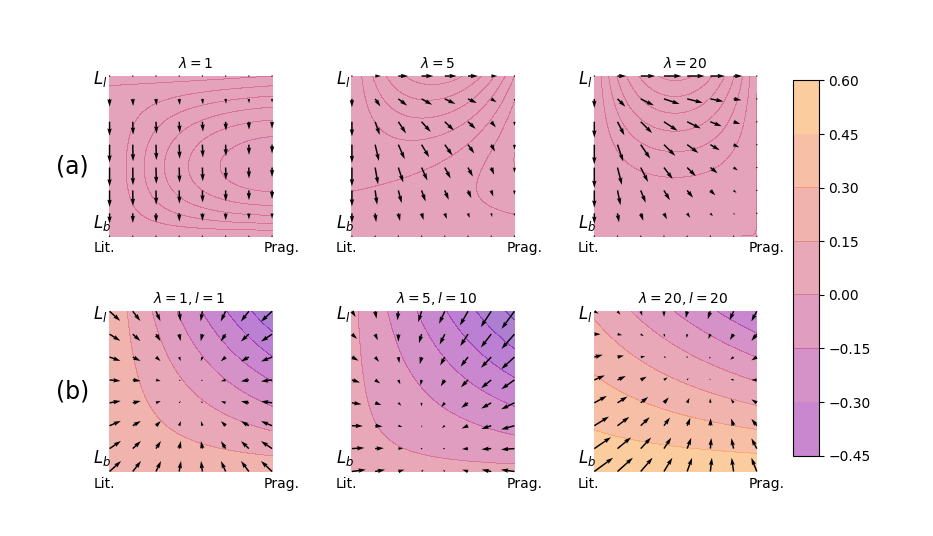
\includegraphics[width=\textwidth,height=8cm, keepaspectratio]{./plots/fig-contourb105k5.png}
\caption{Dynamics on a two-dimensional type space with four types. The $x$-axis represents the proportion of types with $\Llack$; the $y$-axis that of pragmatic ones. Arrows indicate directionality of trajectories after (a) replicator steps and (b) mutator steps with a prior that favors types with $\Llack$ by a factor of $1.05$ over those with $\Lbound$. Colored contours show the proportion of pragmatic $\Llack$ users after a step \tb{I don't think the contours are adding much, so they could be removed. Then again, I think they are rather non-intrusive, look nice, and illustrate how the step-size, depending on where we are in the space, varies.}}

\label{fig:quiver}
\end{figure}

Fig.~\ref{fig:quiver} shows actual evolutionary trajectories in this type space. The replicator steps make the functional disadvantage of $\Llack$ against $\Lbound$ apparent, particularly for its literal users and/or low $\lambda$. They also highlight that the functional difference between literal and pragmatic $\Lbound$ is small. Under functional pressure only, populations move toward the lower part of the square but the steps become small as the lower edge, representing populations composed only  of $\Llack$ users, are reached. As for the mutator diagrams, there are two main things to note. As expected, a small bias for a type will lead to larger proportions to adopt it, provided that likelihood offers little to no differentiation between types. This is the situation the right-most space in Fig.~\ref{fig:quiver} depicts. However, the bias is far from absolute. If, instead, certain types are more likely to be recovered based on the linguistic input they produce, they will be passed on more faithfully. This is why, for instance, populations move toward a majority of $\Llack$-types for $\lambda = 5$ and $l = 10$.


Fig.~\ref{fig:sketch} and \ref{fig:quiver} depict replicator and mutator steps in isolation to better showcase their effects. Their combination will yield different outcomes, which we now turn to in a case study on scalar implicatures. \tb{Also: In this type space RMD way too similar to MD to make it worth the ink. It raises more questions than it answers so I left it out as the plots look identical to those in Fig.~3b}

\subsection{Model summary}

Communicative success and learnability are central to the cultural evolution of language. These
components can be modelled, respectively, as replication based on a measure of fitness in terms
of communicative efficiency and iterated Bayesian learning. Their interaction is described by
the discrete time replicator mutator dynamic in (\ref{eq:RMD_discrete}), repeated here:
\begin{align*}
  x'_i = \sum_j Q_{ji} \frac{x_jf_j}{\sum_h x_h f_h}\,.
\end{align*}
This equation defines the frequency $x'_i$ of type $i$ at the next time step, based on its
frequency $x_i$ before the step, its fitness $f_i$, and the probability that a learner infers
$i$ when observing the behavior of a type-$j$ agent. Fitness-based selection is here thought of
not as biological (fitness as expected relative number of offspring) but cultural (fitness as
likelihood of being imitated or repeated) evolution, since the types that the dynamic operates
on are pairs consisting of a lexicon and a pragmatic use pattern. A type's communicative success depends
on how well it communicates within a population while its learnability depends on the
fidelity by which it is inferred by new generations of learners. The learners' task is
consequently to perform a joint inference over types of linguistic behavior and lexical
meaning.

The model has three parameters: $\lambda$ regulates the degree to which speakers
choose messages that appear optimal from the point of view of the agent's own utility measure
(which may be unrelated to the expected utility when communicating with a given population);
$k$ is the length of observations received by each language learner; $l$ regulates where the learners'
inference behavior lies on a spectrum from probability matching to acquisition of the most likely
teacher type.





\section{Case study: scalar implicatures}
\label{sec:si-case-study}

The model of the previous section formalizes the evolutionary competition between different
sets of lexical representations and ways of using them. This section looks at a case study on
scalar implicatures. It engages in a formal thought experiment to address the
question: if a population of language users could freely combine different lexica with
different dispositions to act on them, what are conditions under which the majority view of scalar
implicatures could have evolved?

Recall that the majority view is that scalar implicatures are non-lexicalized pragmatic
enrichments. Scalar implicature triggers like \emph{some}, \emph{warm} or \emph{may} are
semantically weak expressions for which logically stronger expressions are salient, e.g.,
\emph{all}, \emph{hot} or \emph{must}. For instance, {\em some} is entailed by {\em all}. If
the sentence ``Chris owns all of Johnny Cash's albums'' is true, then ``Chris owns some of
Johnny Cash's albums'' is also true. However, while weaker expressions such as {\em some} are
truth-conditionally compatible with stronger alternatives such as {\em all}, this is not what
their use is normally taken to convey. Instead, the use of a less informative expression when a
more informative one could have been used can license a defeasible inference that stronger
alternatives do not hold (cf. \citealt{horn:1972,gazdar:1979}). In this way, ``Chris owns some
of Johnny Cash's albums'' is strengthened to convey that she owns {\em some but not all}
albums. According to the majority view, this is a pragmatic inference, not part of the
conventional meaning.

In the following we consider a specific application of the model from Section~\ref{sec:model}
which allows us to address the question if or when scalar inferences might (not) lexicalize. We
consider what is perhaps one of the simplest non-trivial setups that speak to this matter and
reflect on its limitations in Section~\ref{sec:discussion}. The setup is introduced in
Section~\ref{sec:setup:-stat-conc}. Section~\ref{sec:simulation-results} describes simulations
and their results.

% Our initial question about the division of labor between semantics and pragmatics can be narrowed to the case of scalar implicatures by asking for a justification for the lack of lexical upper-bounds in weak scalar alternatives. That is, we ask why lexical meanings that lack upper-bounds and convey it pragmatically are regularly selected for over alternatives such as that of codifying the bound semantically. More poignantly, would it not serve language users better if weak(er) expressions such as {\em warm}, {\em or}, {\em some} and {\em big} were truth-conditionally incompatible with stronger alternatives such as {\em hot}, {\em and}, {\em all} and {\em huge} to avoid misunderstanding?  This question is particularly striking considering the number of expressions that license such inferences across natural languages. 

\subsection{Setup}
\label{sec:setup:-stat-conc}

To fill the model from Section~\ref{sec:model} with life, we need to specify the sets of
states, messages and lexica we consider (Section~\ref{sec:stat-mess-conc}). Additionally, we want to
explore the effects of a learning bias in favor of simple lexical representations. One way of
motivating and formalizing such a bias is introduced in Section~\ref{sec:an-induct-learn}.


\subsubsection{States, messages, lexical representations, and lexica} 
\label{sec:stat-mess-conc}


Consider a state space with three states $\States = \set{\snone, \ssome, \sall}$ and think of
it as a partition of possible worlds into cells where none, some or all of the $A$s are $B$s,
for some arbitrary fixed predicates $A$ and $B$. Enlarging the setup from Section~\ref{sec:languages+use} by another state in this way enables us to discern the difference between three kinds of lexica which we will use to unravel the model's dynamics (see below). Eight lexical representations can be distinguished based on their truth or falsity in three world states, six of which are not contradictory or tautological (see Table~\ref{tab:concepts} below).

A lexicon $L$ is a mapping $\Messgs \rightarrow R$ from messages to representations. With three
messages there are $6^3 = 216$ possible lexica. Some assign the same representations to more
than one message and others lexicalize the same representations but associate them with
different messages. Out of these possible lexica, three kinds are of particular
relevance. First, lexica that assign the same lexical representations to more than one
message. Such lexica lack in expressivity but may be favored by particular learning biases
nonetheless (see below). Second, lexica that conventionalize upper-bounds to realize a
one-to-one mapping of messages to states. Finally, lexica that do not lexicalize an upper
bound but allow it to be conveyed pragmatically due to the presence of a stronger lexical
item. There are six lexica of the second kind and six of the third.  The following three lexica
exemplify each kind:
\begin{align*}
  \begin{blockarray}{lccc}
    & & \underline{\Lall} & \\
    & \mygray{\mnone} & \mygray{\msome} & \mygray{\mall} \\
    \begin{block}{l[ccc]}
     \mygray{\snone}  & 0 & 0 & 0\\
     \mygray{\ssome}  & 0 & 0 & 0\\
    \mygray{\sall}   & 1 & 1 & 1\\
    \end{block}
% \\ & & P(\Lall)\rlap{ $\propto 9$} & \\
  \end{blockarray} & &
 \begin{blockarray}{lccc}
    & & \underline{\Lbound} & \\
    & \mygray{\mnone} & \mygray{\msome} & \mygray{\mall} \\
    \begin{block}{l[ccc]}
       & 1 & 0 & 0\\
       & 0 & 1 & 0\\
       & 0 & 0 & 1\\
    \end{block}
%  \\& & P(\Lbound)\rlap{ $\propto 96$} & \\
  \end{blockarray} & &
  \begin{blockarray}{lccc}
    & & \underline{\Llack} & \\
    & \mygray{\mnone} & \mygray{\msome} & \mygray{\mall} \\
    \begin{block}{l[ccc]}
       & 1 & 0 & 0\\
       & 0 & 1 & 0\\
       & 0 & 1 & 1\\
    \end{block}
%   \\& & P(\Llack)\rlap{ $\propto 48$} & \\
  \end{blockarray}
\end{align*}
Lexicon $\Lall$ is clearly bad for communication: all message and interpretation choices will
be equally likely; no information about the observed world state will be conveyed
by its users. In contrast, users of $\Lbound$ can communicate world states perfectly, no matter
whether they are literal or pragmatic users. Users of $\Llack$ can also communicate information
about the actual world state but need pragmatic language use to approximate a one-to-one
mapping between message use and states (see Section~\ref{sec:languages+use}).  

Recall that types are a combination of a lexicon and a manner of language use. We analyze the
model's predictions in populations of types with one of the two behaviors introduced earlier:
literal or pragmatic. The former correspond to level-$0$ reasoners and the latter to level $1$. Accordingly, there is a total of $432$ types. Six types are pragmatic language
users with $\Llack$-like lexica. We refer to these as \emph{target types} because they
represent lexica and language use that conform to the majority view of scalar
implicatures. Twelve types are either literal or pragmatic users of lexica of the
$\Lbound$ kind. We refer to these as \emph{competitor types}, because they are expected to be
the target types' main contenders in evolutionary competition. 

Note that while
different types may lexicalize the same representations, they may nevertheless map different
states to different overt messages. More informally, they speak different languages that
lexicalize the same concepts. Consequently, more often than not different types of the same
kind fail to understand each other.




\subsubsection{An inductive learning bias for semantic simplicity}
\label{sec:an-induct-learn}

There is a growing effort to develop empirically testable representational languages that allow
for the measure of semantic complexity. For instance, so-called {\em languages of thought}
(LOTs) have been put to test in various rational probabilistic models that show encouraging
results (see, e.g., \citealt{katz+etal:2008}, \citeauthor{piantadosi+etal:underreview} under review; 2012, and \citealt{piantadosi+jacobs:2016} for recent discussion). At its
core, a LOT defines a set of operations and composition rules from which lexical representations can be
derived. As a first approximation and for the sake of concreteness, we follow this approach to
motivate and formalize a preference of learners for simpler semantic representations
(\citealt{feldman:2000, chater+vitanyi:2003, piantadosi+etal:2012a,kirby+etal:2015}, \citeauthor{piantadosi+etal:underreview} under review). 
In a weighted generative LOT a representation's complexity is a function of its derivation cost.

\begin{table}
  \centering
  \begin{align*}
    R & \rightarrow_2 R \wedge R 
    & R & \rightarrow_2 \neg R  \\ 
    R & \rightarrow_1 X \subseteq X &
    R & \rightarrow_1 X \neq \emptyset &
    R & \rightarrow_1 X = \emptyset  \\
    X & \rightarrow_1 \set{A,B} & 
    X & \rightarrow_1 X \cap X & 
    X & \rightarrow_1 X \cup X    
  \end{align*}
  \caption{Toy grammar in a set-theoretic LOT with weighted rules.}
  \label{tab:grammar}
\end{table}

Our toy grammar of lexical representations is given in Table~\ref{tab:grammar}. This grammar uses basic
set-theoretic operations to form expressions which can be evaluated as true or false in states
$\snone$, $\ssome$, or $\sall$ from above. Applications of generative rules have a cost attached
to them. Here we simply assume that the formation of Boolean combinations of representations incurs 2
cost units, while all other rule applications incur only 1 cost unit. Table~\ref{tab:concepts}
lists all six lexical representations relevant here, their truth conditions and the simplest formula that
expresses this representation in the grammar in Table~\ref{tab:grammar}.

\begin{table}
  \centering
\begin{center}
  \begin{tabular}{lccclc}
    \toprule
    intuitive name
    & \snone
    & \ssome
    & \sall
    & least complex formula
    & complexity
    \\ \midrule
    ``all''
    & 0
    & 0
    & 1
    & $A \subseteq B$
    & $3$
    \\
    ``some but not all''
    & 0
    & 1
    & 0
    & $A \cap B \neq \emptyset \wedge A \neq \emptyset$
    & $8$
    \\    
    ``some''
    & 0
    & 1
    & 1
    & $A \cap B \neq \emptyset$
    & $4$
    \\
    ``none''
    & 1
    & 0
    & 0
    & $A \cap B = \emptyset$
    & $4$
    \\
    ``none or all''
    & 1
    & 0
    & 1
    & $\neg(A \cap B \neq \emptyset \wedge A \neq \emptyset)$
    & $10$
    \\
    ``not all''
    & 1
    & 1
    & 0
    & $\neg (A \subseteq B)$
    & $5$
    \\
    \bottomrule
  \end{tabular}
\end{center}
\caption{Available lexical representations and their minimal derivation cost.}
\label{tab:concepts}
\end{table}

A complexity measure for lexical representations from Table~\ref{tab:concepts} is used to define a
learning bias that favors simpler representations over more complex ones. The prior probability of a
type is just the prior probability of its lexicon. The prior of a lexicon is a function of the
complexity of the lexical representations in its image set. Lexica with simpler representations accordingly have a
higher prior. One simple way of defining such priors over lexica (and thereby types) is:
\begin{align*}
  P(L)  & \propto \prod_{r \in Im(L)} P(r)   \ \text{, with} & 
  P(r) & \propto \max_{r'}Compl(r') - Compl(r) + 1\,,
\end{align*}
where $Compl(r)$ is the complexity of the minimal derivation cost of representation $r$ according to the
LOT-grammar (see Table~\ref{tab:concepts}). Applied to our space of lexica, this construal assigns the highest probability 
to a lexicon of type $\Lall$, which only uses the simplest lexical representation ``all'' for
all messages. Lexica of type $\Llack$ are less likely, but more likely than $\Lbound$. 

The menu of inductive biases argued to shape language acquisition is steadily being refined. Apart from simplicity, prominent examples include mutual exclusivity \citep{merriman+bowman:1989,clark:2009}, regularization \citep{hudson+etal:2005}, and generalization \citep{smith:2011}. Even when these biases are considered in isolation, there are many ways in which they can be translated into priors over types. The key assumption here, common to all simplicity-biased priors, is that simple representational expressions should be favored over more complex ones (see, e.g., \citealt{goodman+etal:2008, piantadosi+etal:2012a, kirby+etal:2015}). In view of the menu of possible operationalizations, other biases and their potential interplay, we should stress that these details -- from the generative grammar to its complexity measure -- are to be regarded as one convenient operationalization of one general approach to explicating learning biases; this is not a commitment that this general approach is necessarily superior or that, within it, this particular instrumentalization is the single most plausible. We return to this issue in Section~\ref{sec:discussion}.


\subsection{Simulation results}
\label{sec:simulation-results}
Recall that there are three parameters held constant across types: soft-max parameter $\lambda$ affects how strongly
speakers favor messages that appear best from their subjective point of view; the
bottleneck size $k$ influences how faithfully learners can identify their teacher type; $l$
defines the learners' disposition towards choosing the most likely teacher type from the
posterior distribution. We expect that competitor types (types with lexica of the kind
$\Lbound$) have a fitness advantage over target types (pragmatic types with lexica of the kind
$\Llack$), especially for very low levels of $\lambda$ (see Fig~\ref{fig:sketch}). Selection based on fitness alone may
therefore not lead to prevalence of target types in the population. On the other hand, lexica
of type $\Llack$ are simpler than those of type $\Lbound$ by the postulated measure from
above. This may make them more likely to be adopted by learners, especially when $l$ is high. Still, lexica of the kind $\Lall$ are in turn even more likely \emph{a priori} than lexica of the kind $\Llack$. In any case, as showcased in Section~\ref{subsec:example}, the prior is not all that counts for learnability. Simulation results will shed light on the question whether target
types can emerge, and for which parameter constellations.

To better understand the workings of a pressure towards communicative efficiency and a pressure
towards learnability, we look at the behavior of the replicator and mutator step first in
isolation, and then in combination. All simulation runs are initialized with an arbitrary
distribution over types, constituting a population's first generation. All reported results are
the outcome of 50 update steps. These outcomes correspond to developmental plateaus in which
change is, if not absent, then at least very slow. In other words, even if the resulting states
do not correspond to an eventual attracting state, they characterize population states in which the system remains for a long time. As specified in Section~\ref{sec:learnability}, the
mutation matrix $Q$ can be obtained by considering all possible state-message sequences of
length $k$. Given that this is intractable for large $k$, the sets of data which learners are
exposed to are approximated by sampling $250$ $k$-length sequences from each type's production
probabilities.


\subsubsection{Replication only: selection based on communicative success} 

\begin{figure}[t]
\centering
%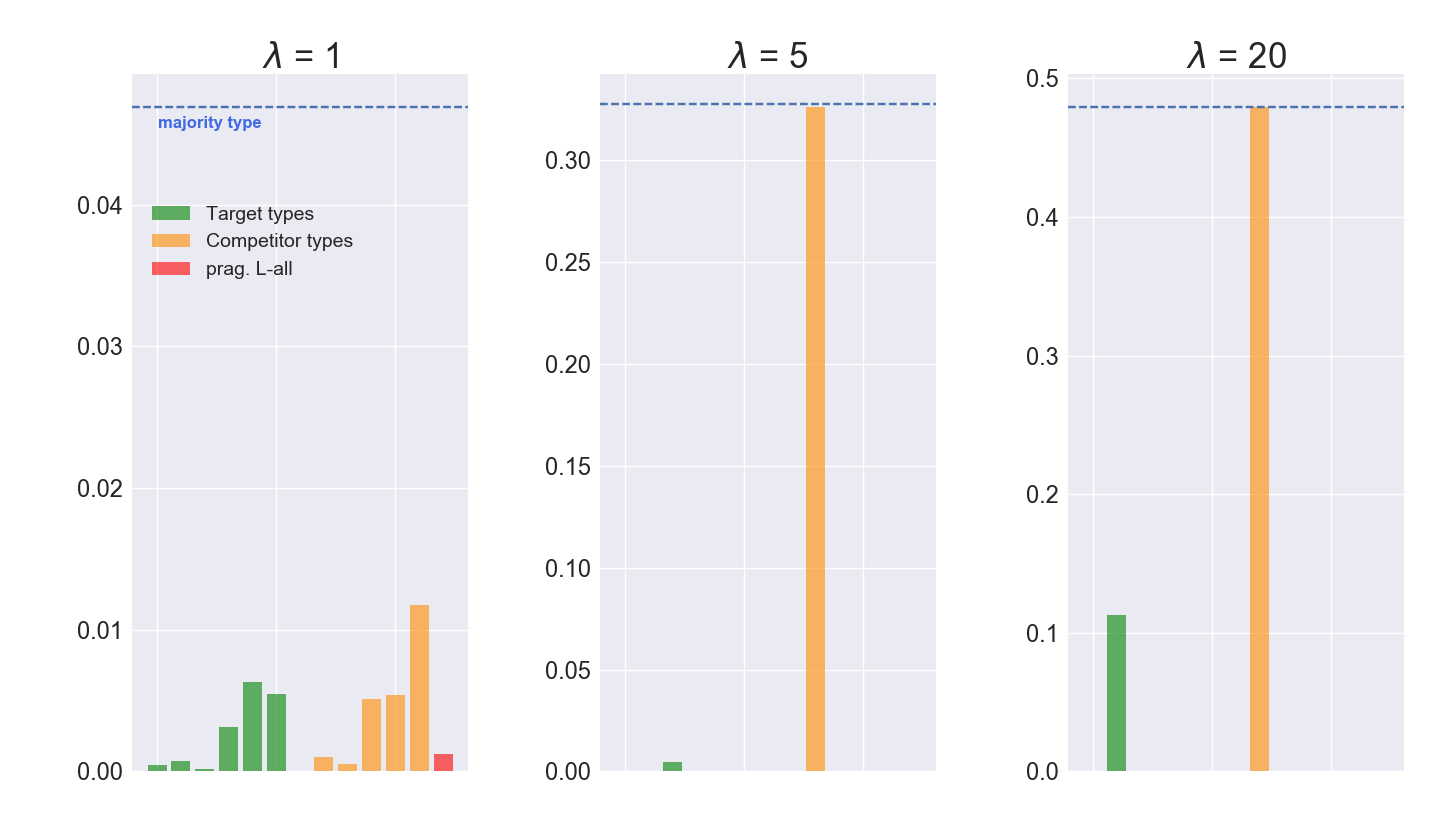
\includegraphics[width=\textwidth,height=8cm, keepaspectratio]{./plots/alt-fig1-onlyr}
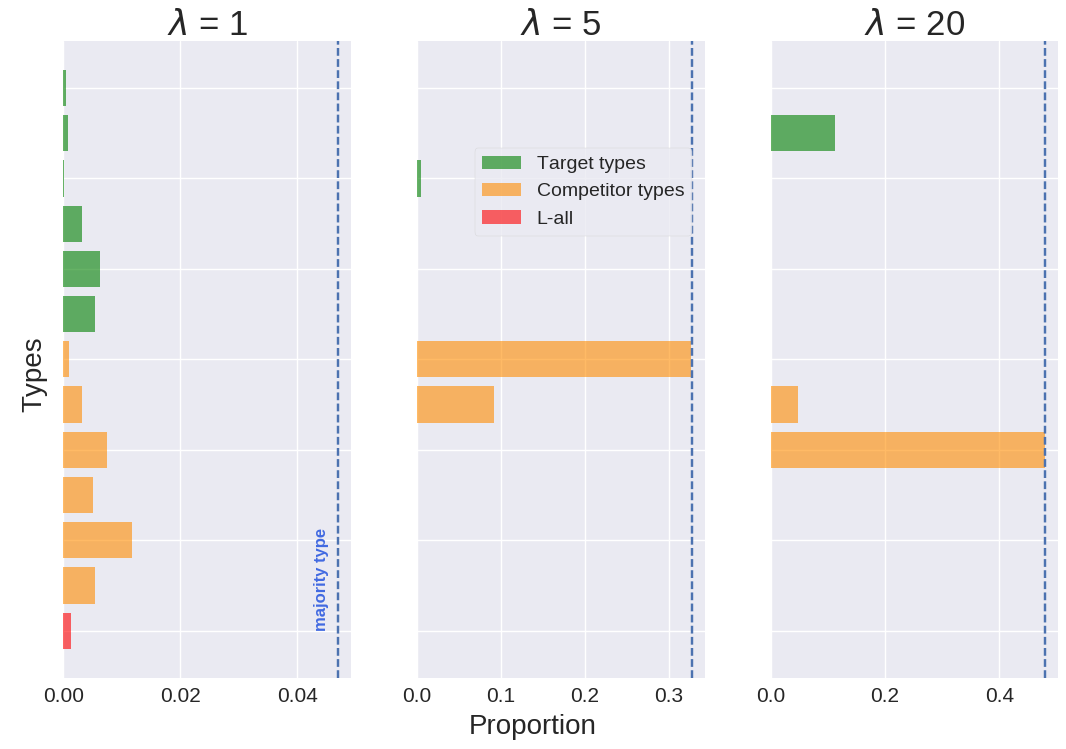
\includegraphics[width=\textwidth,height=8cm, keepaspectratio]{./plots/barh-onlyr}
\caption{Proportion of target types, the six competitor types with the highest proportion, the highest type of the $\Lall$-kind, and the population's majority type, in representative populations after $50$ generations under only a
  pressure for communicative success.}
\label{fig:only-R}
\end{figure}

Selection based on communicative success is sensitive to $\lambda$ since $\lambda$
influences signaling behavior, which in turn determines communicative success. This is
showcased in Fig. \ref{fig:only-R}, which shows the proportion of target types, the highest competitor types and the highest type with $\Lall$ in a representative population after $50$ replicator steps. The plot also indicates the proportion of the
\emph{majority type}: the type with the highest proportion in the population. With
low $\lambda$ many types have very similar behavior, so that evolutionary selection lacks grip
and becomes very slow. The result is a very long transition with near stagnancy in a rather
homogeneous population with many types. Conversely, higher $\lambda$ promotes 
less-stochastic linguistic behavior, widening the gap in expressivity between some types and
promoting more homogeneous populations. As suggested by Fig. \ref{fig:only-R}, the majority
in most populations is not one of the six pragmatic $\Llack$-style types. That is, a pressure
only for communicative success does not lead to a prevalence of target types under any
$\lambda$-value. For instance, with $\lambda = 20$ $1000$ independent populations only had $11$
cases in which the target type was the majority type, corresponding to a mean proportion of
$.003$ across populations. By contrast, in $913$ cases the majority types had $\Lbound$ with,
close to an even share between literal ($454$) and pragmatic types ($459$), corresponding to a
mean proportion of about $.48$ taken together.


\subsubsection{Iterated learning only: transmission fidelity and learnability}

\begin{figure}[t]
\centering
%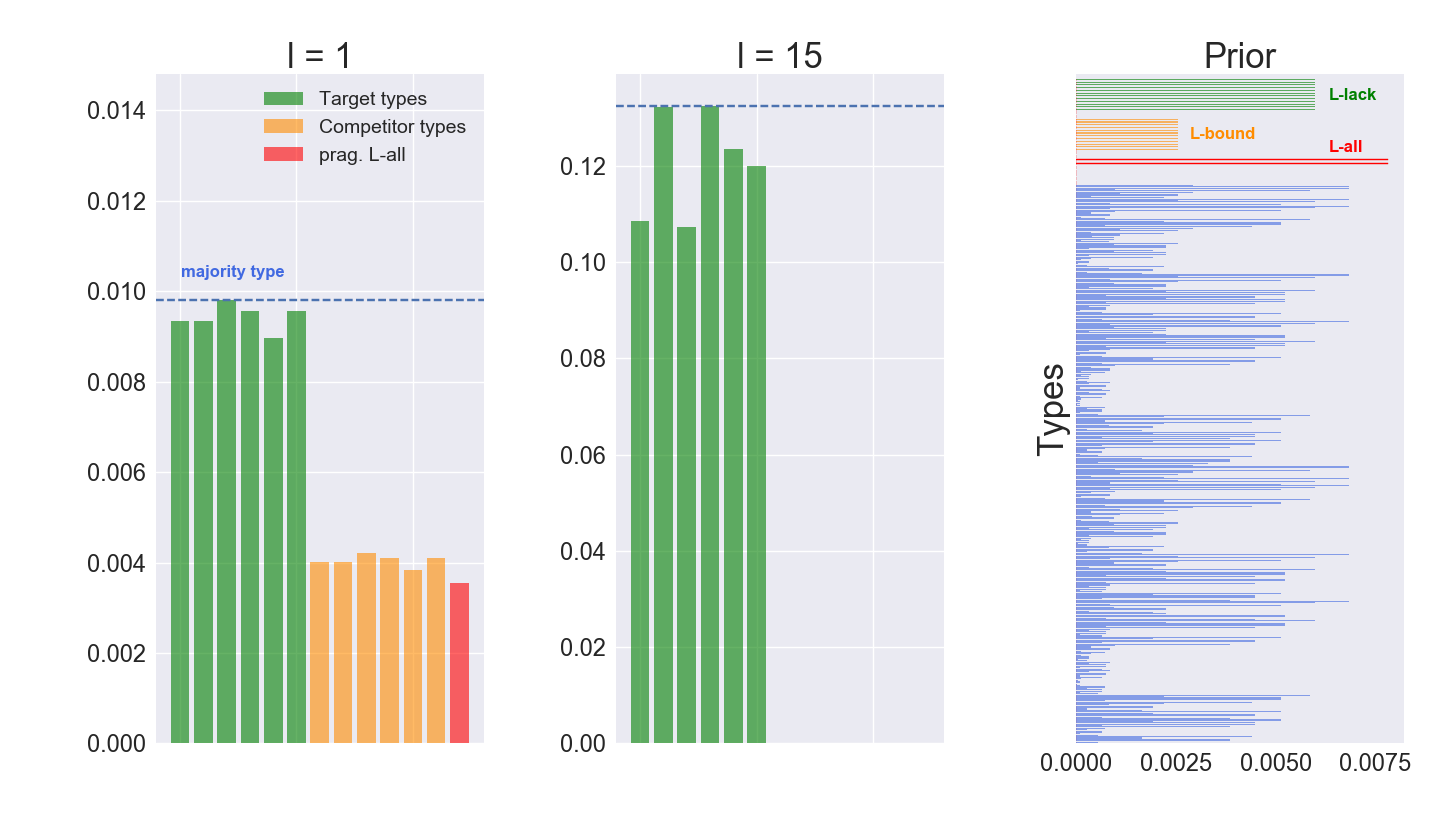
\includegraphics[width=1\textwidth,height=8cm,keepaspectratio]{./plots/alt-fig2-onlym-pr}
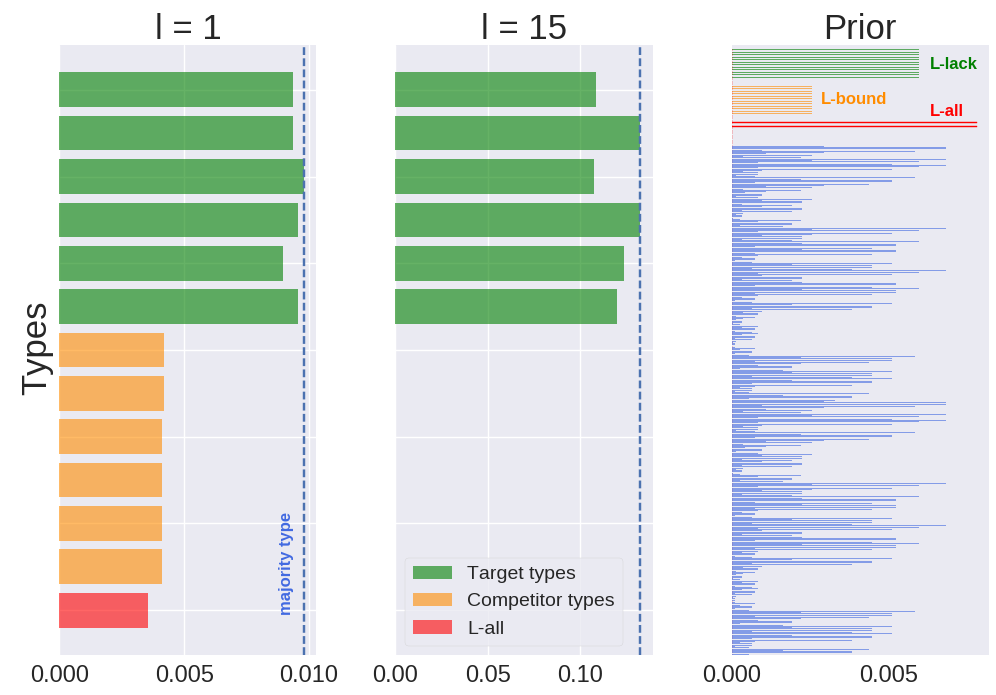
\includegraphics[width=1\textwidth,height=8cm,keepaspectratio]{./plots/barh-onlym}

\caption{Proportion of target types, the six competitor types with the highest proportion, the highest type of the $\Lall$-kind, and the population's majority type in representative populations after $50$ generations under only a
  pressure for learnability ($\lambda = 20, k = 5$). The learning prior is shown in the
  right-most plot with top-most groupings corresponding to types, literal and pragmatic, with
  lexica of kinds $\Llack$, $\Lbound$, and $\Lall$.}
\label{fig:only-M}
\end{figure}

The effect of iterated learning without a pressure for communicative success using either posterior
sampling ($l = 1$) or a stronger tendency towards posterior maximization ($l = 15$) is shown in
Fig.~\ref{fig:only-M} together with the prior over types. The prior shows that while users of
$\Llack$ are not the most favored by the inductive bias (compared, e.g., to $\Lall$) they are
nevertheless more advantaged than others, such as $\Lbound$, in virtue of the relatively simple
semantics they conventionalize (see Section~\ref{sec:an-induct-learn}). Crucially, $\Llack$
enables its users to convey each state with a single message when combined with pragmatic
reasoning and sufficiently high $\lambda$. This makes it less likely to be confused with
other types if the learning data is not too sparse ($k \geq 5$). What is more, learners have
a propensity to infer pragmatic $\Llack$ when the teacher's type produces very similar
data, such as when using $\Lbound$ (see Section~\ref{subsec:example}). Moreover, $\Llack$ is less likely to be confused with
types with different observable behavior because its pragmatic use approximates a one-to-one
form-meaning mapping. As a consequence, a stronger propensity to maximize the posterior
increases their proportion in the population.

However, in contrast to a pressure only for communicative success with high $\lambda$ (see
Fig.~\ref{fig:only-R}), learnability alone does not succeed in selecting for a single
prevalent type; all six target types tend to coexist at roughly equal proportion. Each
is passed on to the next generation with the same faithfulness and, differently from a pressure
for communicative success, they do not stand in competition with each other. In $1000$
independent populations with $\lambda = 20$ all majority types were target types,
with each reaching approximately the same proportion of users in the population.

As with a pressure only for communicative success, low values of $\lambda$ make the differences in observable behavior across types less pronounced. This makes differences in the likelihood of particular types having generated a learning input less pronounced. Therefore, low $\lambda$ leads populations to reflect the learners' inductive bias more faithfully. This favors functionally deficient but a priori preferred types such as those that use  $\Lall$. A pressure for learnability alone may consequently lead to a spread of communicatively suboptimal types that lexicalize simpler semantics. In the extreme, when $l = 1$ and $\lambda = 1$ all
of $1000$ independent populations had users of $\Lall$ as majority types. For higher $\lambda$, it becomes clear that a high prior is not the only thing that counts when it comes to learnability (see Section~\ref{subsec:example}). As soon as there is information for learners to discern whether one type is more likely to have generated the data (depending on $\lambda$ and $k$), it becomes paramount for types to produce data that makes them easily identifiable if they are to be inferred more often.


\subsubsection{Combining pressures of communicative success and learnability}

Pressure for communicative success and learnability are not sufficient on their own to have a
single target type dominate the population. When pressured for communicative success, the  communicative advantage of $\Lbound$ users leads to their prevalence. When pressured for
learnability, pragmatic $\Llack$ is promoted over functionally similar but semantically more
complex alternatives such as $\Lbound$. However, learnability alone does not foment the
propagation of a single target type across the population.

\begin{figure}[t]
\centering
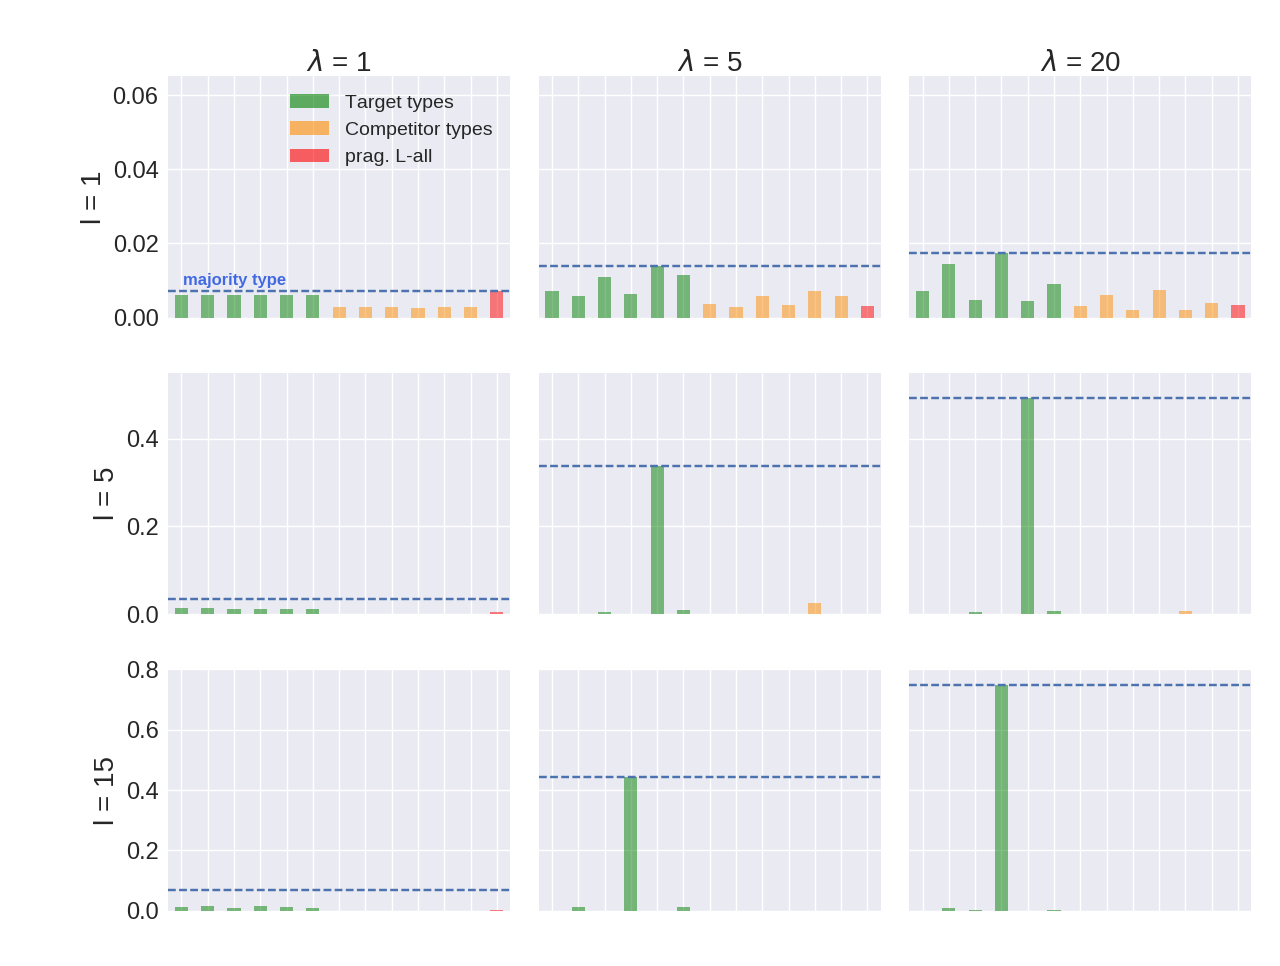
\includegraphics[width=1\textwidth,height=8cm,keepaspectratio]{./plots/alt-fig3-r+m}
\caption{Proportion of target types, the six competitor types with the highest proportion, the highest type of the $\Lall$-kind, and the population's majority type in representative populations after $50$ generations under both pressures ($k = 5$).}
\label{fig:rmd}
\end{figure}

Fig. \ref{fig:rmd} illustrates the combined effects of both pressures for a sample of
$\lambda$ and $l$ values. These results show that an inductive learning bias for simpler
semantics in tandem with functional pressure can lead to the selection of a single target
type, and so to a division of labor between semantics and pragmatics.
The proportion of a single majority target type increases with $\lambda$ and
$l$. Pressure for communicative success magnifies the effects of iterated learning and dampens
the proliferation of multiple types of a kind, equal in expressivity and learnability. A pressure towards learnability favors the transmission of simpler semantics and thereby indirectly selects for pragmatic language use in these types. Pragmatic behavior, however, is not necessarily selected for in types that can do away without pragmatic reasoning such as $\Lbound$ users (see Section~\ref{subsec:example}). 

As before, low $\lambda$ and $l$ lead to the prevalence of communicatively suboptimal types
that are a priori favored, such as $\Lall$. An increase in $\lambda$ leads to the selection of
target types but does not lead to monomorphic populations if learners sample from the posterior (see the uppermost row in Fig.~\ref{fig:rmd}). Finally, a combination of high $\lambda$ and $l$ leads to increasing proportions of a single majority target type. This joint influence is summarized in Fig. \ref{fig:diff}, which shows the mean difference between the highest target type and the highest proportion of a type of a different kind in $1000$ independent populations across $\lambda$ and $l$ values. Higher values of $\lambda$ and $l$ increase the prevalence of a single target type, whereas lower values lead to less pronounced differences, with a valley resulting from low $\lambda$ and high $l$ (cf. Fig. \ref{fig:rmd} with $\lambda = 1$ and $l=15$). 

\begin{figure}[t]
\centering
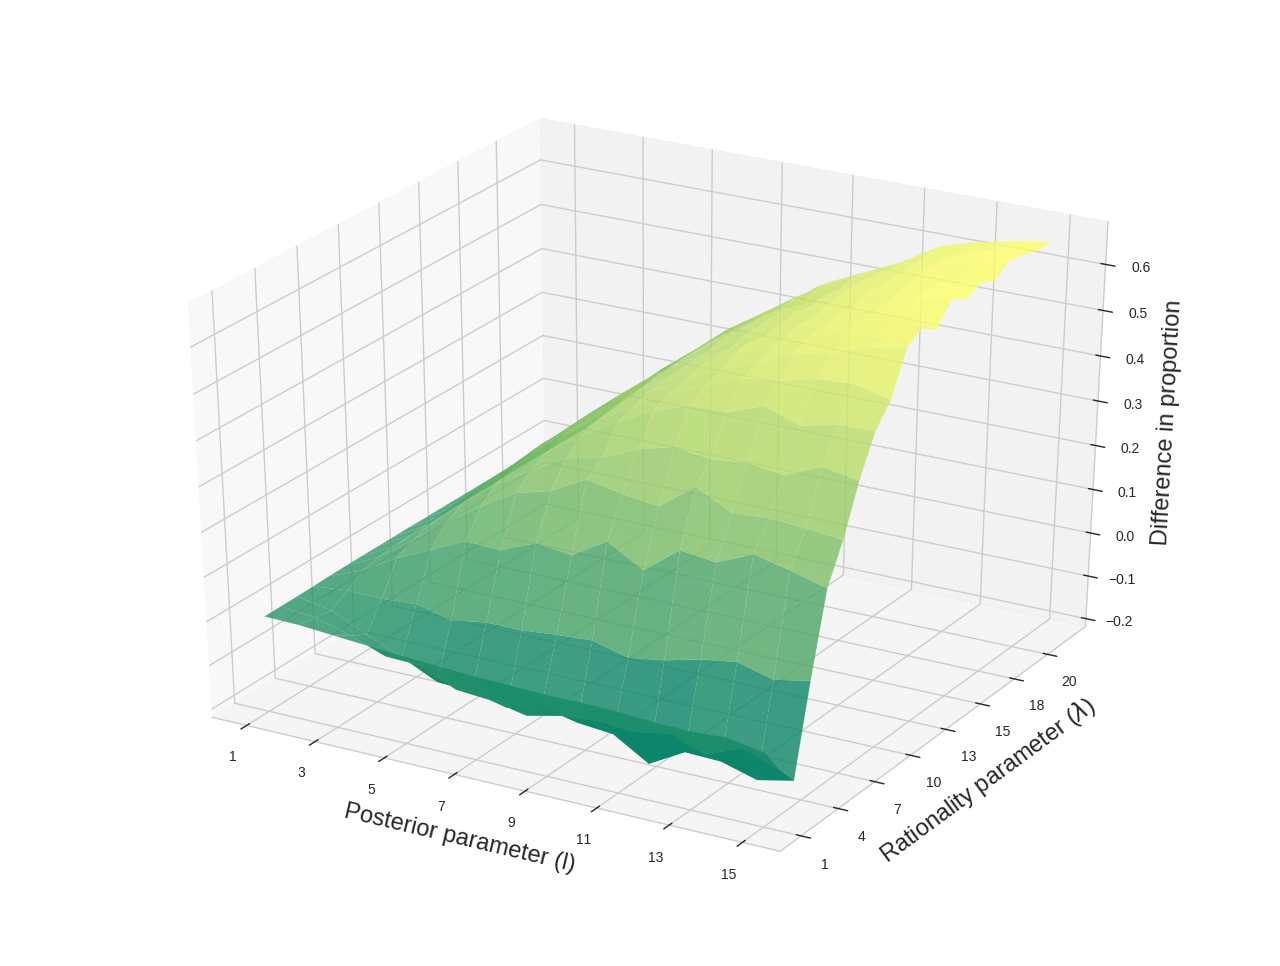
\includegraphics[width=1\textwidth,height=10cm,keepaspectratio]{./plots/fig4-3d-incumbents-difference} %alternatively without '-3d'
\caption{Mean difference between proportion of highest target type and highest other type in
  $1000$ independent populations after $50$ generations under both pressures ($k = 5$).}
\label{fig:diff}
\end{figure}

Effects of manipulating the sequence length $k$ have not been addressed so far, but are rather
predictable: small values lead to more heterogeneous populations that reflect the learner's
prior more faithfully. This is due to the fact that the likelihood that a small sequence was
produced by any type is relatively uniform (modulo prior). By contrast, larger values
increasingly allow learners to differentiate types with different signaling behaviors.

When pressured for communicative success only, target types are outcompeted by competitor types. When pressured for learnability, populations are polymorphic due to lack of competition; minimally among types of a kind. However, due to the prior, learners that are exposed to the input of either targets or competitors tend to acquire the former. The consequence of combining both pressures is then that the (slight) functional disadvantage of targets is counterbalanced by an advantage in learnability. This leads to large proportions of targets in a population and, due to the competition among types applied by each replicator steps, to more monomorphic populations. 

To recapitulate, other than the involvement of pressure on both communicative success and learnability,
the resulting proportion of pragmatic $\Llack$ speakers primarily hinges on three
factors. First, the degree, captured by $\lambda$, to which agents try to maximize
communicative success from their own subjective point of view. Second, the inductive bias,
which leads learners to prefer simpler over more complex semantic representations in
acquisition. Lastly, the learning behavior, captured by parameter $l$, where approximating a
MAP strategy magnifies the effects of the learning bias in tandem with replication. 


More broadly, target types, which represent the majority view of scalar implicatures, can come to
dominate the population if three assumptions are met: (i) language is pressured toward both
communicative success {\em and} learnability; (ii) pragmatic language use is an option; (iii) learners prefer
simpler over more complex lexical representations and exhibit a tendency towards the
acquisition of the type that best explains the learning data.


\section{General discussion}\label{sec:discussion}
The approach introduced here combines game-theoretic models of functional pressure towards
successful communication \citep{nowak+krakauer:1999}, effects of transmission perturbations on
(iterated) language learning \citep{griffiths+kalish:2007}, probabilistic speaker and listener
types of varied degrees of pragmatic sophistication \citep{frank+goodman:2012,
  franke+jaeger:2014} as well as reasoning about unobservable lexical representations
\citep{bergen+etal:2012,bergen+etal:2016}. This allows for a conceptual investigation of the
(co-)evolution of conventional meaning and pragmatic language use. Main contributions of the
model are (i) its modular separation of communicative success and learnability on evolutionary
trajectories, (ii) the characterization of language learning as a joint inference over
linguistic behavior and lexical meaning, and (iii) the possibility to trace the co-evolution of
conventional semantics and pragmatic use.

With respect to (i), \citet{kirby+etal:2015} propose a comparable model of the interaction
between a lexicon's expressivity and its learnability. A main difference is that here we
considered communicative pressure for mutual understanding. This pressure can indirectly select for expressive types, those that can convey states unequivocally, whereas Kirby et al. only consider the bearing that the latter ability has on the production of learnable data. We see three main reasons for considering communicative success rather than just
expressivity, and for looking at communication and learning rather than just learning. First, learning alone can  promote populations with non-negligible proportions of functionally defective types. This is true both of simulations, e.g., our $\Lall$-types in Fig.~\ref{fig:only-M}, as well as of laboratory experiments with human subjects (see \citealt{kirby+etal:2008,silvey+etal:2014}, and see \citealt{fay+etal:2013} for review of laboratory results). Second and more importantly, types may be equally expressive but their performance as means of information transfer crucially depend not only on themselves but on the population they find themselves in (compare the competition of target types in Fig. 
\ref{fig:rmd} and their lack of competition in Fig. \ref{fig:only-M}). That is, we contend that adopting an expressive type that generates learnable data does not, in itself, capture a type's arguably central communicative function of transferring information to peers. Taking communication into consideration allows the model to be responsive to the task for which language is learned. Lastly, chains of iterated learning alone do not put types in direct competition. Accordingly, learning leads to polymorphous populations in which multiple types of a kind coexist \citep{nowak:2006}. 

The main result of our case study is that types that correspond to the majority view of scalar
implicatures -- scalar readings are non-lexicalized pragmatic enrichments -- can come to dominate a
population. This can happen if pragmatic language use is recruited indirectly by a preference for simpler lexical representations (relative to more complex ones that lead to comparable overt linguistic behavior without pragmatic language use). Under this view, semantics
and pragmatics play a synergic role: pragmatic use allows maintenance of simpler representations;
pressure towards representational simplicity indirectly promotes pragmatic over literal
language use. As a consequence, iterated transmission and use of language lead to a
regularization that may explain the lack of lexicalization of systematic pragmatic enrichments.

While the results of this case study are interesting, they also raise a number of critical
issues. First of all, while many favorable parameter settings exist which lead to a prevalence
of target types, other types are usually represented in non-negligible proportions (see Fig.~\ref{fig:rmd} and \ref{fig:diff}). This may
just be a technical quirk of the mutator step; but there is a related issue of empirical
importance. Several experimental studies on scalar implicatures suggest that participants can
be classified as either semantic or pragmatic users of, in particular, \emph{some}
\citep[e.g.,][]{BottNoveck2004:Some-Utterances,NieuwlandDitman2010:On-the-incremen,DegenTanenhaus2012:Processing-Scal}. The
former consistently accept \emph{some} where \emph{all} would be true as well, the latter do
not. Interestingly, in our simulations when a target type is the majority type an inflated
proportion of the population uses compatible lexica with a lexicalized upper
bound. Particularly in those parameter settings where the prior influences the outcome less. In
other words, we do find a tendency toward a similar co-existence of semantic and pragmatic
types. Whether this analogy has any further explanatory value is an interesting path for future
exploration.

Another important issue that is not addressed in the model are potential costs associated with
pragmatic reasoning. Here, we simply assumed that literal and pragmatic reasoning strategies
exist from the start and are equally costly to apply. In contrast, empirical results suggest
that the computation of a scalar implicature may involve additional cognitive effort
\citep[e.g.,][]{BrehenyKatsos2006:Are-Generalised,deNeys+schaeken:2007,huang+snedeker:2009,Jr.Bailey2013:Possibly-all-of}. Extensions
of the model presented here to include processing costs for pragmatic language use would be
interesting future work. It seems plausible that effects of reasoning cost may trade off with
the frequency with which a given scalar expression is used. It may be that frequently drawn
scalar implicatures lexicalize to avoid cost, whereas infrequent ones are derived on-line to
avoid more complex lexical representations during acquisition. Such a prediction would lend itself to
empirical testing in line with a recent interest in differences between various scalar
implicature triggers \citep{Tielvan-TielMiltenburgvan-Miltenburg2014:Scalar-Diversit}. 

Our case study could be criticized as follows: all it shows is that scalar implicatures do not
lexicalize because upper bounds are dispreferred lexical representations. This criticism would be too
superficial and highly unjust. Dispreferred lexical representations can thrive under evolutionary
selection. Lexicalized upper-bounds can dominate a population because they may boost
communicative success. But they do not have to. Moreover, as stressed throughout this investigation, even without selective pressure
for communicative success, it is not necessarily the case that the types that are most
likely \emph{a priori} will dominate. The dynamics of iterated learning are not that
trivial. Iterated learning does not necessarily promote the \emph{a priori} more likely type,
but tends to promote a type $t$ based on a gradient of how many other types might likely mutate
into $t$, so to speak. Taken together, without an explicit model of the interaction between
pressure for communicative success and learnability, it is far from trivial to judge whether or when
preferred or dispreferred representations can be adaptive. This is why a major contribution of this
paper is the arrangement of many different ingredients into a joined model of the (co-)evolution
of lexical meaning and pragmatic use. 

What is more, it is not that we just assumed a prior disadvantage of lexicalized upper
bounds. We tried to motivate and formalize a general assumption about lexical representations'
complexity with a concrete, albeit provisional proposal. The specification of a learning bias
in terms of a ``grammar of representations'' can and should be seen critically, however. Much
depends on the primitives of such a grammar. For instance, the lexical representation ``none or
all'' is the most complex in Table~\ref{tab:concepts}. But consider adding a new primitive
relation between sets $A \smile B$ which is true if and only if
$\neg(A \cap B \neq \emptyset \wedge A \neq \emptyset)$. The lexical representation ``none or
all'' would then be one of the simplest. Clearly, further research, empirical and conceptual,
into the role of representational complexity, processing costs and learning biases is
needed. The model here makes a clear and important contribution nonetheless: it demonstrates
how simplicity of representations can interact with use and evolutionary selection and shows
that for simple representations to emerge it may require pragmatic strategies to compensate
their potential expressive deficiencies. Hence a model of co-evolving semantics and pragmatics is
needed. Future work should also include the possibility that representational simplicity may
itself be a notion that is subject to evolutionary pressure
\citep[cf.][]{ThompsonKirby2016:Culture-Shapes-}, as well for the evolution of elements that define
the agents' cognitive make-up; $\lambda$ and $l$.

Finally, this case study should not be interpreted as a proposal for a definite explanation of
how scalar implicatures evolved. Other factors should be considered eventually even if they
will lead to much more complex modeling. One such factor is the observation that
non-lexicalized upper bounds allow a broader range of applicability. For example, when the speaker is
not certain as to whether \emph{all} is true. This may suggest an alternative and purely
functionalist argument for why upper-bounded meanings do not conventionalize: should contextual
cues provide enough information to the hearer to identify whether a bound is intended to be
conveyed pragmatically, then this is preferred over expressing it overtly through longer
expressions. For example, by saying {\em some but not all} explicitly. Importantly, although
morphosyntactic disambiguation may be dispreferred due to its relative length and complexity
\citep{piantadosi+etal:2012b}, it allows speakers to enforce an upper-bound and override
contextual cues that might otherwise mislead the hearer. In a nutshell, this explanation posits that scalar implicatures fail to lexicalize because, all else being equal, speakers prefer to communicate as economically as possible and pragmatic reasoning enables them to do so. What this alternative argument does not explain is why functional pressure does not lead to the emergence of different, equally costly lexical items to express different knowledge states of the speaker (\citealt[252-267]{horn:1984}, 
\citealt{horn:1972,traugott:2004,vdAuwera:2010}). For instance, to the emergence of two expressions for each weak scalar expression; one with and one lacking an upper-bound. That is, this argument does not explain why English and other languages do not have a monomorphemic dual for, e.g., {\em some} that lexicalizes an upper-bound. If this hypothetical expression existed, it could be deployed to signal that the speaker knows that {\em some but not all} holds, and unbounded {\em some} could exclusively signal epistemic uncertainty. Looking at pressure from learnability might come in again. 

Beyond scalar implicatures, the model can generate predictions about likely lexicalization trajectories of pragmatic inferences, or a lack thereof. In this realm an interesting issue is whether proposed principles, such as the semantic conventionalization of once highly context-dependent inferences if they become regular enough \citep{levinson:2000,traugott:2004}, can be given
a formal rationale and inform postulated directionalities of change. The present investigation made a first start and gave a framework for exploring these issues systematically.


\section{Conclusion}
The cultural evolution of meaning is influenced by intertwined pressures. We set out to
investigate this process by putting forward a model that combines pressure toward successful
information transfer with perturbations that may arise in the transmission of linguistic
knowledge in acquisition. Its objects of selection and replication are pairs of lexical
meanings and patterns of language use. This allows the model to trace the evolutionary interaction between
conventional meaning and pragmatic use. Additionally, it takes the challenge seriously of
neither semantics nor pragmatics being directly observable. Instead, learners need to infer
these unobservables from overt data that results from their combination.  These components and
their mutual influence were highlighted in a case study on the lack of lexical upper-bounds in
weak scalar expression. This study showed that, when pressured for learnability and communicative
success, the former force can drive for simpler semantic representations inasmuch as pragmatics
can compensate for lack of expressivity in use. That is, the relative learning advantage of
simpler semantics in combination with functional pressure in use may offer an answer to why
natural languages fail to lexicalize systematic pragmatic inferences. And, more broadly, lead to a
division of labor between semantics and pragmatics.

\bibliographystyle{chicago}
\bibliography{./bounds-rmd}




\end{document}
